\documentclass[aip,jcp,reprint,floatfix]{revtex4-2}

\usepackage[utf8]{inputenc}
\usepackage[T1]{fontenc}
\usepackage{amsmath}
\usepackage{graphicx}
\usepackage{booktabs}
\usepackage{multirow}
\usepackage{makecell}
\usepackage{adjustbox}

\usepackage{amsmath,amssymb,mathtools}
\usepackage{bm}

\usepackage{siunitx}
\sisetup{detect-all}

\usepackage{chemformula}
\usepackage[version=4]{mhchem}

\usepackage{pgfplots}
\pgfplotsset{compat=1.18}

\usepackage{xcolor}
\usepackage{tikz}
\usetikzlibrary{positioning,arrows.meta,shapes.geometric}
\usetikzlibrary{calc}

\usepackage{orcidlink}

\usepackage{placeins}   % permette \FloatBarrier se serve

\setlength{\tabcolsep}{3pt}

\newcommand{\vect}[1]{\bm{#1}}
\newcommand{\rank}{\operatorname{rank}}

\begin{document}

\title{Tensor Representation and Transport of Centrifugal Distortion Constants: A Representation-Independent Framework}

\author{Vincenzo Barone\,\orcidlink{0000-0001-6420-4107}}
\affiliation{INSTM, via G. Giusti 9, 50121 Firenze, Italy}
\email{vincebarone52@gmail.com}

%Centrifugal distortion constants are recast as projections of underlying 
%tensorial objects, enabling representation-independent transport and revealing 
%the onset of nonlinear effects.

\begin{abstract}
Centrifugal distortion constants in Watson's effective rotational
Hamiltonian are not uniquely defined physical observables, as their
numerical values depend on the chosen Hamiltonian reduction and axis
representation. This representation dependence complicates comparisons
between parametrizations and between theory and experiment.

In this work, centrifugal distortion constants are recast as
projections of underlying tensorial objects encoding the intrinsic
rovibrational structure of the system. Within this formulation,
spectroscopic parameters $W$ are expressed as projections of tensor
representatives $T$ ($W = P T$), where $P$ is a representation-dependent
projection operator. Since this mapping is not invertible in general,
tensor representatives are reconstructed via the Moore--Penrose
pseudoinverse, implemented through a numerically stable singular value
decomposition (SVD), which provides a well-defined and robust gauge
fixing of the inverse problem.

This enables a lift--transport--reprojection procedure in which
representation changes are performed at the tensor level and mapped
back to the desired parametrization. A central result is that standard
quartic and sextic centrifugal distortion constants can be consistently
interpreted within a common tensorial sector generated by combinations
of the first derivatives of the inverse inertia tensor. Within this
sector, different Watson parametrizations correspond to alternative
projections of the same underlying tensorial object.

Here, the linearity refers to the mapping between tensor representatives
and spectroscopic parameters, which remains linear even when
anharmonic contributions arising from cubic force constants are
included. These contributions extend the physical content of the model
without introducing additional independent tensorial degrees of freedom
in the mapping to spectroscopic parameters.

The formulation also identifies the first intrinsic breakdown of this
structure, arising from the $H_{22}$ contribution at the quartic level,
and provides simple diagnostics to quantify deviations from the linear
transport regime. As a result, representation changes reduce to
well-defined linear operations in tensor space, enabling a consistent
and representation-independent comparison and interpretation of
spectroscopic parameters.

Applications to representative molecular systems demonstrate that the
tensor framework rationalizes the behavior of spectroscopic parameters
across different parametrizations and provides a practical and
scalable route for their analysis, comparison, and interpretation.
\end{abstract}

\maketitle

\section{Introduction}

High-resolution rotational spectroscopy provides some of the most
precise structural information available for isolated molecules and
offers direct access to their rovibrational dynamics.
\cite{TownesSchawlow1955,GordyCook1984,BunkerJensen2005}
Gas-phase rotational and rovibrational spectra encode equilibrium
geometries, vibrational couplings, and subtle electronic effects with
remarkable accuracy. Modern microwave and millimeter-wave techniques
now enable high-resolution investigations of increasingly complex
systems, including flexible organic molecules, reactive intermediates,
and species of atmospheric and astrochemical relevance.

As molecular size increases, however, rotational spectra become
progressively more congested, making their assignment and
interpretation increasingly challenging. Reliable analyses therefore
require support from quantum-chemical calculations capable of
providing accurate rotational and rovibrational parameters. At the
same time, the theoretical description of high-resolution spectra is
computationally demanding, requiring accurate equilibrium structures,
high-order derivatives of the potential energy surface, and the
inclusion of anharmonic and rotation--vibration couplings. These
ingredients scale unfavorably with system size, so that simplified
models based on rigid-rotor and harmonic approximations are still
widely employed, leading at best to semi-quantitative predictions.

The analysis of rotational spectra is commonly performed using
Watson's effective rotational Hamiltonian,
\cite{Watson1968,Watson1977,Watson1968JCP,AlievWatson1976}
which incorporates quartic and sextic centrifugal distortion terms to
account for rotation--vibration coupling. Within this framework,
centrifugal distortion constants are obtained from least-squares fits
of measured transition frequencies and are expressed in a chosen
Hamiltonian reduction ($A$ or $S$) and principal-axis representation
($I$, $II$, or $III$).

A fundamental limitation of this description is that centrifugal
distortion constants are not unique physical observables. Their
numerical values depend explicitly on the adopted Hamiltonian
reduction and axis representation. Although different parametrizations
describe the same underlying rovibrational dynamics, their equivalence
is not transparent at the level of the fitted constants. As a result,
transformations between reductions or axis systems may produce large
variations in individual parameters, obscuring the relation between
different parametrizations and complicating comparisons between
experiment and theory.

This representation dependence is not merely a formal issue, but has
direct practical consequences. It affects the comparison of
spectroscopic datasets, the interpretation of fitted parameters, and
the validation of quantum-chemical predictions. In particular,
differences between parameter sets may reflect either genuine physical
effects or artifacts of the chosen parametrization, and disentangling
these contributions is often nontrivial.

Despite the long-standing use of Watson-type Hamiltonians and the
availability of explicit transformation formulas, existing approaches
remain formulated at the level of spectroscopic parameters themselves.
As a consequence, they do not provide a representation-independent
description of centrifugal distortion, nor a systematic way to separate
intrinsic rovibrational content from parametrization-dependent effects.

The problem becomes even more pronounced in the context of
quantum-chemical predictions. Centrifugal distortion constants can be
computed from rovibrational perturbation theory
\cite{Franke2021}
or extracted from variational rovibrational calculations.
\cite{Dinu2022,BowmanCarterHuang2003,MatyusCzakoCsaszar2009,
JensenBunker2000,BunkerJensen2005}
However, variational approaches provide transition energies that must
be fitted to obtain spectroscopic parameters, while perturbative
treatments typically rely on predefined molecular orientations that do
not necessarily coincide with the spectroscopic representations used in
experimental analyses. A consistent and representation-independent
framework is therefore required to relate spectroscopic constants
obtained in different parametrizations and to connect them reliably
with theoretical predictions.

The situation is particularly critical for sextic centrifugal
distortion constants. While perturbative treatments of vibrational
anharmonicity are widely available, complete rovibrational
implementations remain comparatively rare and are generally limited to
small systems.
\cite{BowmanCarterHuang2003,MatyusCzakoCsaszar2009,
Jensen1988MORBID,JensenBunker2000,BunkerJensen2005}
In practice, sextic constants are often available only within specific
implementations, and no general procedure exists for transporting them
consistently between Hamiltonian representations. The representation
problem is therefore both conceptual and operational.

While tensorial and operator-based formulations of rovibrational Hamiltonians 
have been discussed in various contexts, a unified identification of quartic 
and sextic centrifugal distortion constants as projections of a common 
underlying tensorial structure has not, to our knowledge, been explicitly 
established. In particular, no general operational procedure has been 
formulated to reconstruct such tensorial objects from spectroscopic 
parameters and to transport them consistently across different Hamiltonian 
parametrizations.

In the present work, we introduce a tensorial formulation in which
centrifugal distortion constants are recast as projections of
underlying tensor representatives encoding the intrinsic
rovibrational structure of the system. In this perspective, Watson
parameters are not treated as fundamental quantities, but as
representation-dependent projections of a common underlying object.

The key operational step is the reconstruction of these tensor
representatives from spectroscopic parameter sets via the
Moore--Penrose pseudoinverse.
\cite{Penrose1955}
In practice, this reconstruction is performed using a singular value
decomposition (SVD), which ensures numerical stability, filters
ill-conditioned directions in parameter space, and isolates the
physically meaningful tensor subspace. This choice corresponds to the
minimum-norm tensor compatible with the available data and represents
the least-structured tensor consistent with the input, thereby avoiding
the amplification of null-space components and providing a natural
gauge fixing of the inverse problem.

Within this formulation, changes of Hamiltonian reduction or axis
representation are no longer performed directly on Watson parameters.
Instead, they are carried out through a three-step
lift--transport--reprojection procedure: the tensor representative is
first reconstructed (lift), then transformed under permutations of the
principal axes or representation changes (transport), and finally
projected back onto the desired parametrization (reprojection). This
separates the intrinsic rovibrational content from the
representation-dependent parametrization and reduces representation
changes to linear operations in tensor space.

The overall structure of the framework is illustrated in
Figure~\ref{fig:workflow}. Starting from a set of spectroscopic
parameters, tensor representatives are reconstructed through
pseudoinverse lifting, transported under representation changes, and
finally reprojected onto the desired Hamiltonian parametrization.
Optional harmonic information enables the evaluation of diagnostic
quantities that probe the validity of the linear tensor approximation.

\begin{figure*}[ht]
\centering

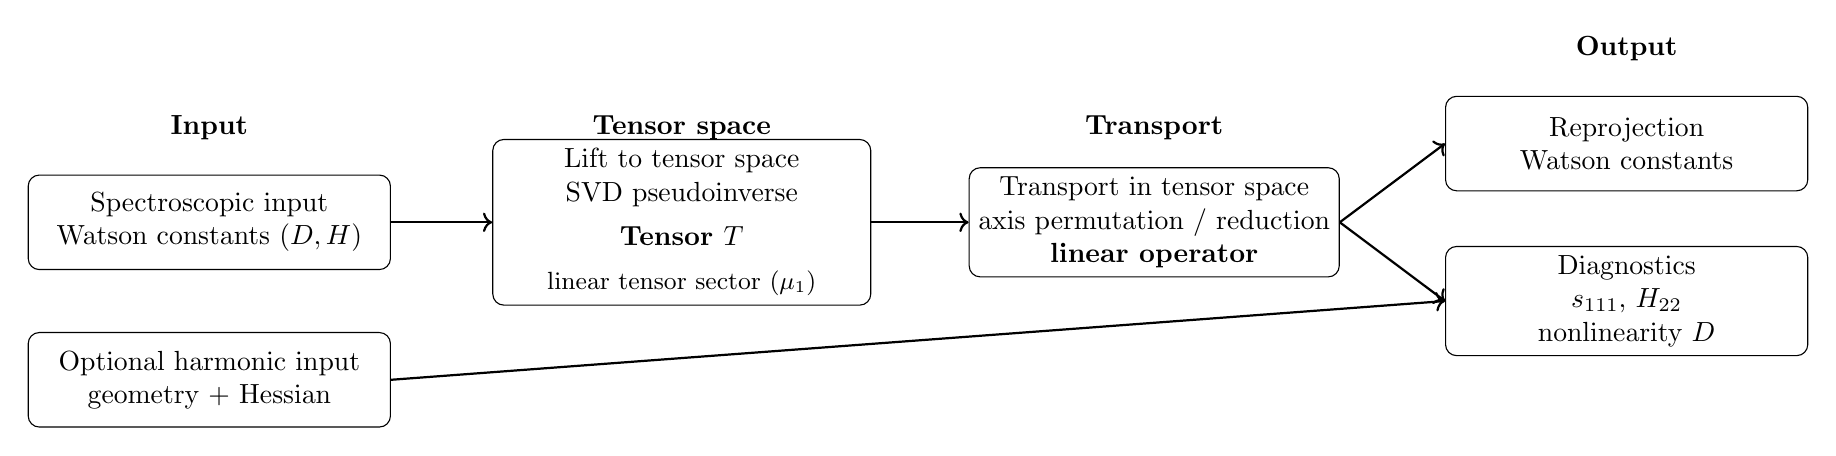
\begin{tikzpicture}[
box/.style={
rectangle,draw,rounded corners,
align=center,
minimum width=4.6cm,
minimum height=1.2cm
},
core/.style={
rectangle,draw,rounded corners,
align=center,
minimum width=4.8cm,
minimum height=1.4cm
},
arrow/.style={->, thick}
]

% =======================
% LEFT COLUMN (INPUT)
% =======================

\node[box] (fit) at (0,0)
{Spectroscopic input\\Watson constants $(D,H)$};

\node[box] (harm) at (0,-2)
{Optional harmonic input\\geometry + Hessian};

\node[draw=none] at (0,1.2) {\textbf{Input}};

% =======================
% CENTER (TENSOR)
% =======================

\node[core] (tensor) at (6,0)
{Lift to tensor space\\
SVD pseudoinverse\\[4pt]
\textbf{Tensor $T$}\\[4pt]
{\small linear tensor sector ($\mu_1$)}};

\node[draw=none] at (6,1.2) {\textbf{Tensor space}};

% =======================
% TRANSPORT
% =======================

\node[box] (transport) at (12,0)
{Transport in tensor space\\
axis permutation / reduction\\
\textbf{linear operator}};

\node[draw=none] at (12,1.2) {\textbf{Transport}};

% =======================
% OUTPUT
% =======================

\node[box] (reproj) at (18,1)
{Reprojection\\Watson constants};

\node[box] (diag) at (18,-1)
{Diagnostics\\$s_{111}$, $H_{22}$\\nonlinearity $D$};

\node[draw=none] at (18,2.2) {\textbf{Output}};

% =======================
% ARROWS
% =======================

\draw[arrow] (fit.east) -- (tensor.west);
\draw[arrow] (tensor.east) -- (transport.west);
\draw[arrow] (transport.east) -- (reproj.west);
\draw[arrow] (transport.east) -- (diag.west);
\draw[arrow] (harm.east) -- (diag.west);

\end{tikzpicture}

\caption{
Operational structure of the tensor framework. Spectroscopic parameters are lifted to a representation-independent tensor space via SVD-based pseudoinverse reconstruction, defining tensor representatives within the linear sector generated by $\mu_1$. Representation changes are performed as linear operations in tensor space, and the results are reprojected onto the desired Watson parametrization. Optional harmonic input enables the evaluation of diagnostic quantities that probe the breakdown of the linear tensor regime.
}

\label{fig:workflow}
\end{figure*}



A central result of this work is that standard quartic and sextic
centrifugal distortion constants belong to a common tensorial sector.
This sector can be formally identified as the space generated by
quadratic and higher-order combinations of the first derivatives of
the inverse inertia tensor ($\mu_1$), and is closed with respect to the
projection mapping onto spectroscopic parameters. Within this sector,
different Watson parametrizations correspond to alternative projections
of the same underlying tensorial object, providing a unified description
of centrifugal distortion that is independent of the chosen representation.

Here, the term ``linear'' refers to the mapping between tensor
representatives and spectroscopic parameters, while the tensorial sector
itself is generated by nonlinear combinations of $\mu_1$.

Within this framework, anharmonic contributions arising from cubic force
constants extend the physical content of the model without introducing
additional independent tensorial degrees of freedom in the mapping to
spectroscopic parameters. In this sense, the tensorial sector remains
effectively closed under the standard quartic and sextic contributions
routinely included in
rovibrational perturbation theory.

The first intrinsic departure from this structure occurs at the
quartic level through the $H_{22}$ contribution, which introduces a
second-level geometric tensor beyond the $\mu_1$-generated sector and
therefore defines the onset of a genuinely nonlinear regime within the
standard perturbative framework.

This decomposition also leads to simple and computationally inexpensive
diagnostics. In particular, scalar indicators derived from the
tensorial structure quantify deviations from the linear transport
regime and provide predictive information on the sensitivity of
centrifugal distortion constants to Hamiltonian representation.

An implementation of the present framework is provided through the
CeDiTT (Centrifugal Distortion Tensorial Transformation) program,
which enables the practical application of the
lift--transport--reprojection procedure to both experimental and
theoretical datasets. By combining tensor reconstruction with SVD-based
regularization, CeDiTT allows robust comparison, transport, and
validation of centrifugal distortion constants across different
representations, with the currently implemented operational features
summarized in Appendix~E.

The goals of the present work are therefore threefold. First, we
introduce an operational procedure for transforming centrifugal
distortion constants between Hamiltonian representations through
tensor reconstruction, transport, and reprojection. Second, we identify
the minimal tensorial sector underlying the standard quartic and
sextic constants, clarifying the structural origin of their
representation dependence. Third, we introduce tensorial diagnostics
that quantify and interpret deviations from this transport picture.

The resulting formulation establishes a direct connection between the
tensorial objects underlying centrifugal distortion and the
spectroscopic parameters appearing in Watson Hamiltonians. In
computational spectroscopy, rovibrational couplings derived from
quantum-chemical force fields determine the underlying tensorial
structure, while in experimental spectroscopy the same structure can be
reconstructed from fitted Watson constants. This establishes a unified
framework for the analysis, comparison, and interpretation of
centrifugal distortion constants across different representations.

The theoretical framework underlying these results is developed in the
following section, where the tensor representation is constructed from
the rovibrational Hamiltonian and leads naturally to the
lift--transport--reprojection procedure.


\section{Theoretical Framework}

The central idea of this work is that centrifugal-distortion constants
should be treated as projections of underlying tensorial objects,
rather than as fundamental quantities tied to a specific Hamiltonian
representation. Within this perspective, the rovibrational structure
of the system is encoded in a hierarchy of tensorial quantities, while
the spectroscopic parameters correspond to representation-dependent
projections of this underlying structure.

The organization of this hierarchy is illustrated schematically in
Figure~\ref{fig:tensor_hierarchy}. At the lowest level, the equilibrium
geometry defines the inertia tensor and its inverse, whose first 
derivatives with respect to normal coordinates ($\mu_1$) generate
a minimal tensorial sector underlying standard quartic and sextic
centrifugal distortion. This sector is constructed from quadratic and
higher-order combinations of $\mu_1$ and is characterized by a linear
mapping to spectroscopic parameters.

Higher-order contributions, arising from second-order geometric terms
and anharmonic force constants, extend the physical content of the
description. Importantly, anharmonic contributions associated with
cubic force constants remain within the same tensorial sector in the
sense that they do not introduce additional independent tensorial
degrees of freedom in the mapping to spectroscopic parameters. In
contrast, genuinely new tensorial structure appears only beyond this
level, defining the first intrinsic departure from the linear regime.

\begin{figure*}[ht]
\centering

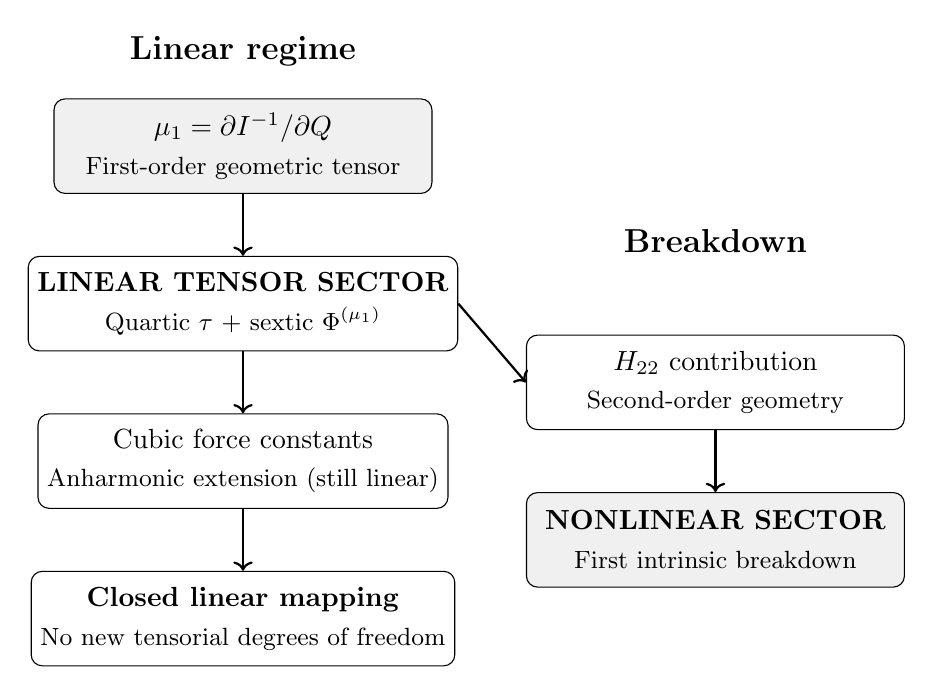
\begin{tikzpicture}[
box/.style={
rectangle,draw,rounded corners,
align=center,
minimum width=4.8cm,
minimum height=1.2cm
},
core/.style={
rectangle,draw,rounded corners,
align=center,
minimum width=4.8cm,
minimum height=1.2cm,
fill=gray!12
},
arrow/.style={->, thick}
]

% =======================
% LEFT COLUMN (LINEAR SECTOR)
% =======================

\node[core] (mu1) at (0,0)
{$\mu_1 = \partial I^{-1} / \partial Q$ \\[2pt]
\small First-order geometric tensor};

\node[box] (linear) at (0,-2)
{\textbf{LINEAR TENSOR SECTOR} \\[2pt]
\small Quartic $\tau$ + sextic $\Phi^{(\mu_1)}$};

\node[box] (cubic) at (0,-4)
{Cubic force constants \\[2pt]
\small Anharmonic extension (still linear)};

\node[box] (closed) at (0,-6)
{\textbf{Closed linear mapping} \\[2pt]
\small No new tensorial degrees of freedom};

% =======================
% RIGHT COLUMN (BREAKDOWN)
% =======================

\node[box] (h22) at (6,-3)
{$H_{22}$ contribution \\[2pt]
\small Second-order geometry};

\node[core] (nonlinear) at (6,-5)
{\textbf{NONLINEAR SECTOR} \\[2pt]
\small First intrinsic breakdown};

% =======================
% ARROWS
% =======================

\draw[arrow] (mu1) -- (linear);
\draw[arrow] (linear) -- (cubic);
\draw[arrow] (cubic) -- (closed);

\draw[arrow] (linear.east) -- (h22.west);
\draw[arrow] (h22) -- (nonlinear);

% =======================
% LABELS
% =======================

\node at (0,1.2) {\large \textbf{Linear regime}};
\node at (6,-1.2) {\large \textbf{Breakdown}};

\end{tikzpicture}

\caption{
Conceptual organization of centrifugal-distortion contributions within the tensor framework. The first derivatives of the inverse inertia tensor ($\mu_1$) generate a linear tensor space that fully determines both standard quartic and sextic centrifugal distortion constants. Anharmonic contributions arising from cubic force constants extend the physical content while remaining within the same linear mapping, so that the linear sector remains closed. The first intrinsic breakdown arises from the $H_{22}$ contribution, which introduces a second-level geometric tensor and defines the onset of a nonlinear tensor sector.
}

\label{fig:tensor_hierarchy}

\end{figure*}


The derivation of this tensor formulation requires a sequence of
intermediate developments, which are introduced in the following
sections before the final representation is established.


\subsection{Rovibrational Hamiltonian and perturbative structure}

The starting point of the present formulation is the perturbative
structure of the rovibrational Hamiltonian. Expanding in powers of
vibrational normal coordinates $Q_k$ and rotational angular momentum
operators $J_\alpha$, one writes
\begin{equation}
H = \sum_{r,v} H_{rv},
\end{equation}
where the indices $r$ and $v$ denote the degree in rotational angular
momentum and vibrational coordinates, respectively.

Within the standard Watson partition, the blocks
\begin{equation}
H_{03}, \quad H_{12}, \quad H_{30}
\end{equation}
are treated as first-order contributions, whereas
\begin{equation}
H_{40}, \quad H_{22}, \quad H_{13}, \quad H_{31}, \quad H_{04}
\end{equation}
enter at second order. These terms define the perturbative channels
that generate centrifugal-distortion effects in the effective
Hamiltonian.

The effective Hamiltonian is obtained through a Van Vleck contact
transformation,\cite{VanVleck1932}
\begin{equation}
\tilde{H} = e^{iS} H e^{-iS},
\end{equation}
whose Baker--Campbell--Hausdorff (BCH) expansion\cite{Baker1905,Campbell1897,Hausdorff1906} systematically generates rotation--vibration couplings and their higher-order contributions.

At quartic and sextic order, the relevant channels include
\begin{equation}
\begin{aligned}
H_{12}H_{12}, \quad H_{22}, \quad H_{12}H_{30}, \quad H_{30}H_{12}, \\
H_{12}H_{12}H_{12}, \quad H_{12}H_{03}, \quad H_{03}H_{03}.
\end{aligned}
\end{equation}

Among these contributions, the $H_{12}H_{12}$ channel generates the
standard quartic tensor, while the $H_{22}$ term introduces the first
departure from the linear tensor sector discussed above. Higher-order
channels, involving cubic force constants and mixed rotation--vibration
terms, contribute to the sextic tensor and define the next level of the
tensorial hierarchy.


\subsection{Inverse inertia and quartic tensors}

The rotational kinetic energy is governed by the inertia tensor $I$,
or equivalently by its inverse
\begin{equation}
\mu = I^{-1}.
\end{equation}

Within the present formulation, the fundamental quantity is not the
inertia tensor itself, but its first derivative with respect to
vibrational coordinates. Differentiation of $I^{-1} I = 1$ yields
\begin{equation}
\frac{\partial I^{-1}}{\partial Q_k}
=
- I^{-1} \frac{\partial I}{\partial Q_k} I^{-1},
\end{equation}
which defines the first-order tensor
\begin{equation}
\mu^{(k)}_{\alpha\beta}
=
\frac{\partial (I^{-1})_{\alpha\beta}}{\partial Q_k}
=
- \sum_{\gamma\delta}
\mu_{\alpha\gamma}
\left(
\frac{\partial I_{\gamma\delta}}{\partial Q_k}
\right)
\mu_{\delta\beta}.
\end{equation}

The set of tensors $\{\mu^{(k)}\}$, hereafter denoted collectively as
$\mu_1 \equiv \partial I^{-1}/\partial Q$, generates the minimal linear
tensor space underlying standard centrifugal-distortion effects.

Within the standard Watson formulation, the quartic contribution to the
effective Hamiltonian reads
\begin{equation}
H^{(4)}_{\mathrm{std}} =
H_{40}
-
H_{12} H_{02}^{-1} H_{12},
\end{equation}
which leads to the quartic tensor
\begin{equation}
\tau_{\alpha\beta\gamma\delta}
=
- \frac{1}{2}
\sum_k
\frac{
\mu^{(k)}_{\alpha\beta}
\mu^{(k)}_{\gamma\delta}
}{\omega_k^2},
\label{eq:tau_std}
\end{equation}
showing explicitly that the standard quartic tensor depends exclusively
on $\mu_1$.

To make this dependence more explicit, let $\mathbf{r}_i$ be Cartesian
coordinates and $\mathbf{l}_{ik}$ the normal-mode displacement vectors:
\begin{equation}
\mathbf{r}_i = \mathbf{r}_i^{(0)} + \sum_k Q_k \mathbf{l}_{ik}.
\end{equation}

The inertia tensor is
\begin{equation}
I_{\alpha\beta}
=
\sum_i m_i
\left(
r_i^2 \delta_{\alpha\beta}
-
r_{i\alpha} r_{i\beta}
\right),
\end{equation}
and its derivative reads
\begin{equation}
\frac{\partial I_{\alpha\beta}}{\partial Q_k}
=
\sum_i m_i
\left[
2 (\mathbf{r}_i \cdot \mathbf{l}_{ik}) \delta_{\alpha\beta}
-
l_{ik,\alpha} r_{i\beta}
-
r_{i\alpha} l_{ik,\beta}
\right].
\end{equation}

An equivalent and numerically more stable implementation can be built
from Coriolis-type first-level quantities derived from the same
harmonic model. In the present work, however, the explicit tensorial
formulation is kept in terms of $\mu_1=\partial I^{-1}/\partial Q$,
since this is the representation used uniformly in the quartic,
sextic, and post-standard channels discussed below.

This result shows that the entire standard quartic sector is fully
determined by $\mu_1$, without introducing additional geometric degrees
of freedom.


\subsection{Explicit sextic tensor}

For the purposes of the present work, the sextic tensor is reformulated
in terms of first-order inverse-inertia derivatives and cubic force
constants, without introducing intermediate quantities such as $c_1$
and $c_2$.\cite{Watson1968} This representation does not follow the
standard Watson decomposition, but is algebraically equivalent and is
adopted here to make the tensorial structure and its computational
organization more transparent.

This choice is motivated by three key aspects. First, it makes explicit
that the standard sextic tensor does not involve the second derivative
of the inverse inertia tensor $\mu_2$. Second, it provides a natural
separation between geometric contributions, entirely determined by
$\mu_1$, and anharmonic contributions arising from cubic force
constants. Third, it distinguishes contributions with different
computational cost, separating terms involving two-mode couplings from
those requiring the full three-mode cubic force field.

Within this formulation, the sextic tensor is written as
\begin{equation}
\Phi_{\alpha\beta\gamma\delta\epsilon\zeta}
=
\Phi^{(\mu_1)}_{\alpha\beta\gamma\delta\epsilon\zeta}
+
\Phi^{(3,2)}_{\alpha\beta\gamma\delta\epsilon\zeta}
+
\Phi^{(3,3)}_{\alpha\beta\gamma\delta\epsilon\zeta},
\end{equation}
where each term corresponds to a distinct physical and computational
contribution.

To make the harmonic scaling explicit, we introduce the mode-rescaled
first-level tensor
\begin{equation}
\mathcal{M}^{(i)}_{ab}
=
\omega_i^{3/2}\widetilde{\mu}^{(i)}_{ab},
\end{equation}
so that the quartic tensor reads
\begin{equation}
\tau_{abcd}
=
-2\sum_i
\frac{\mathcal{M}^{(i)}_{ab}\mathcal{M}^{(i)}_{cd}}{\omega_i^2}.
\end{equation}
This already shows that the standard sextic geometry sector generated
from quartic insertions is homogeneous of order $\omega^{-4}$, whereas
the explicit cubic sector is expected to be homogeneous of order
$\omega^{-3}$ when written in terms of reduced cubic force constants.

The Coriolis-dressed first-level quantity entering the sextic geometry
sector is
\begin{equation}
\widetilde{\nu}^{(i)}_{abc}
=
\sum_j
\frac{2}{3}\,
\frac{\omega_i^2+2\omega_j^2}{\omega_i^{5/2}\omega_j^2}
\Big[
B_a\,\zeta_{aij}\,\mathcal{M}^{(j)}_{bc}
+
B_b\,\zeta_{bij}\,\mathcal{M}^{(j)}_{ca}
+
B_c\,\zeta_{cij}\,\mathcal{M}^{(j)}_{ab}
\Big],
\end{equation}
so that the geometric sextic sector is written entirely in terms of
$\tau$, $\widetilde{\nu}$, and the first-level tensor space generated
by $\mu_1$.

For the dominant diagonal sextic component one obtains
\begin{equation}
\Phi_{aaa}=X_1-X_2+X_3+X_4,
\end{equation}
with
\begin{align}
X_1 &= \frac{3}{16}\sum_x\frac{\tau_{aaax}^2}{B_x},&
X_2 &= \frac{1}{2}\sum_i \omega_i\left(\widetilde{\nu}^{(i)}_{aaa}\right)^2,\\
X_3 &= \frac{1}{6}\sum_{i,j,k}
\frac{\Phi^{(3),\mathrm{red}}_{ijk}}{\omega_i\omega_j\omega_k}\,
\mathcal{M}^{(i)}_{aa}\mathcal{M}^{(j)}_{aa}\mathcal{M}^{(k)}_{aa},&
X_4 &= \frac{1}{4}\sum_{x\neq a}
\frac{\tau_{xaaa}^2}{B_a-B_x}.
\end{align}
Here $X_1$, $X_2$, and $X_4$ belong to the geometric sector and are of
order $\omega^{-4}$, whereas $X_3$ is linear in the reduced cubic force
constants and is of order $\omega^{-3}$.

The cubic contribution itself separates naturally into a semi-diagonal
sector and a genuine three-index sector,
\begin{equation}
X_3=X_3^{(2)}+X_3^{(3)},
\end{equation}
with
\begin{align}
X_3^{(2)}
&=
\frac{1}{6}\sum_i
\frac{\Phi^{(3),\mathrm{red}}_{iii}}{\omega_i^3}
\left(\mathcal{M}^{(i)}_{aa}\right)^3
+\frac{1}{2}\sum_{i\neq j}
\frac{\Phi^{(3),\mathrm{red}}_{iij}}{\omega_i^2\omega_j}
\left(\mathcal{M}^{(i)}_{aa}\right)^2\mathcal{M}^{(j)}_{aa},
\\
X_3^{(3)}
&=
\sum_{i<j<k}
\frac{\Phi^{(3),\mathrm{red}}_{ijk}}{\omega_i\omega_j\omega_k}
\mathcal{M}^{(i)}_{aa}\mathcal{M}^{(j)}_{aa}\mathcal{M}^{(k)}_{aa}.
\end{align}

This decomposition makes transparent both the perturbative hierarchy
and the computational hierarchy: the standard sextic geometry is
carried entirely by first derivatives of $I^{-1}$, the two-index cubic
sector is controlled by the semi-diagonal constants $\Phi^{(3)}_{iii}$
and $\Phi^{(3)}_{iij}$, and the three-index sector requires the full
set of genuine $\Phi^{(3)}_{ijk}$ couplings.

This explicit reformulation is, to our knowledge, not visible in the
usual $c_1/c_2$ presentation of the standard sextic problem. In the
present form the first-level tensorial origin of the standard sextic
sector, its $\omega^{-4}/\omega^{-3}$ hierarchy, and the separation
between semi-diagonal and genuine three-index cubic contributions all
become manifest.

The same partition is directly parallel to the standard VPT2
vibration--rotation corrections $\alpha_{i,a}$ to the rotational
constants. For each mode $i$ and principal axis $a$ one may write
\begin{equation}
\alpha_{i,a}
=
\alpha^{\mathrm{Cor}}_{i,a}
+
\alpha^{\mathrm{In}}_{i,a}
+
\alpha^{\mathrm{Anh}}_{i,a},
\end{equation}
with the non-resonant Coriolis term
\begin{equation}
\alpha^{\mathrm{Cor}}_{i,a}
=
-\frac{2 B_a^2}{\omega_i}
\sum_{j\ne i}
\zeta_{aij}^2\,
\frac{3\omega_i^2+\omega_j^2}{\omega_i^2-\omega_j^2},
\end{equation}
the inertial contribution
\begin{equation}
\alpha^{\mathrm{In}}_{i,a}
=
-\frac{3 B_a^2}{2\omega_i}
\sum_b
\frac{1}{I_b}
\left(
\frac{\partial I_{ab}}{\partial Q_i}
\right)^2,
\end{equation}
or, equivalently,
\begin{equation}
\alpha^{\mathrm{In}}_{i,a}
=
-\frac{3 B_a^2 I_a^2}{2\omega_i^4}
\sum_b
I_b\,
\left(\mathcal{M}^{(i)}_{ab}\right)^2,
\end{equation}
which shows that the geometric part of the vibration--rotation
correction is likewise homogeneous of order $\omega^{-4}$. The
anharmonic correction is
\begin{equation}
\alpha^{\mathrm{Anh}}_{i,a}
=
-2\pi\sqrt{\frac{c\,m_u}{h}}\,
B_a^2
\left[
\frac{\Phi^{(3),\mathrm{red}}_{iii}}{\omega_i^{3/2}}\,
\frac{\partial I_{aa}}{\partial Q_i}
+
\sum_{j\ne i}
\frac{\Phi^{(3),\mathrm{red}}_{iij}}{\omega_j^{3/2}}\,
\frac{\partial I_{aa}}{\partial Q_j}
\right].
\end{equation}
In the present CeDiTT implementation this is the operational
backend-faithful form of the standard VPT2 anharmonic correction,
written so as to make explicit that only the semi-diagonal cubic
constants $\Phi^{(3)}_{iii}$ and $\Phi^{(3)}_{iij}$ enter.
Using the principal-axis identity
\begin{equation}
\frac{\partial I_{aa}}{\partial Q_j}
=
-I_a^2\mu^{(j)}_{aa}
=
-I_a^2\frac{\mathcal{M}^{(j)}_{aa}}{\omega_j^{3/2}},
\end{equation}
the anharmonic term can be rewritten as
\begin{equation}
\alpha^{\mathrm{Anh}}_{i,a}
=
2\pi\sqrt{\frac{c\,m_u}{h}}\,
B_a^2 I_a^2
\left[
\frac{\Phi^{(3),\mathrm{red}}_{iii}}{\omega_i^3}\,
\mathcal{M}^{(i)}_{aa}
+
\sum_{j\ne i}
\frac{\Phi^{(3),\mathrm{red}}_{iij}}{\omega_j^3}\,
\mathcal{M}^{(j)}_{aa}
\right],
\end{equation}
which makes the $\omega^{-3}$ scaling of the cubic VPT2 correction
fully explicit. In other words, the anharmonic $\alpha$ correction
involves the same ingredients as the two-index cubic sector of the
sextic tensor, namely first derivatives of $I^{-1}$, Coriolis
couplings, and the semi-diagonal cubic constants $\Phi^{(3)}_{iii}$
and $\Phi^{(3)}_{iij}$, but not the genuine three-index constants
$\Phi^{(3)}_{ijk}$ with $i<j<k$. This makes the computational
hierarchy explicit: the low-cost cubic information required for
vibration--rotation corrections is the same low-cost information that
controls the semi-diagonal sextic sector, whereas the genuine
three-mode cubic force field enters only at the next level.

The corresponding explicit expressions for the mixed classes
$\Phi_{aab}$ and $\Phi_{abc}$, together with the full backend-faithful
partition of the standard sextic tensor and its projection formulas,
are collected in Appendices~B and~C.


\subsection{Hierarchy of linearity breakdown}

The linear tensor sector defined by $\mu_1$ provides a complete
description of centrifugal distortion at the standard quartic and
sextic levels. The first intrinsic departure from this linear
structure arises at quartic order from the $H_{22}$ contribution,
which originates from the second-order expansion of the inverse
inertia tensor in the rotational kinetic energy.

Starting from
\begin{equation}
T_{\mathrm{rot}} = \frac{1}{2} \sum_{\alpha\beta}
\mu_{\alpha\beta}(Q) J_\alpha J_\beta,
\end{equation}
and expanding $\mu_{\alpha\beta}(Q)$ up to second order in normal
coordinates,
\begin{equation}
\mu_{\alpha\beta}(Q)
=
\mu_{\alpha\beta}
+
\sum_k \mu^{(k)}_{\alpha\beta} Q_k
+
\frac{1}{2} \sum_{k,l} \mu^{(kl)}_{\alpha\beta} Q_k Q_l,
\end{equation}
one obtains the exact second-order contribution
\begin{equation}
H_{22}
=
\frac{1}{4}
\sum_{\alpha\beta}
\sum_{k,l}
\mu^{(kl)}_{\alpha\beta}
\, Q_k Q_l \,
J_\alpha J_\beta.
\end{equation}

The second derivative of the inverse inertia tensor is
\begin{equation}
\mu^{(kl)} =
\frac{\partial^2 I^{-1}}{\partial Q_k \partial Q_l}.
\end{equation}

Using
\begin{equation}
\frac{\partial^2 I^{-1}}{\partial Q_k \partial Q_l}
=
- I^{-1} \frac{\partial^2 I}{\partial Q_k \partial Q_l} I^{-1}
+ 2 I^{-1} \frac{\partial I}{\partial Q_k} I^{-1}
\frac{\partial I}{\partial Q_l} I^{-1},
\end{equation}
one obtains
\begin{equation}
\mu_2 = B(\mu_1) - N,
\end{equation}
where the bilinear term
\begin{equation}
B(\mu_1) =
2 I^{-1}
\left(\frac{\partial I}{\partial Q_k}\right)
I^{-1}
\left(\frac{\partial I}{\partial Q_l}\right)
I^{-1},
\end{equation}
depends exclusively on $\mu_1$, while
\begin{equation}
N =
I^{-1}
\frac{\partial^2 I}{\partial Q_k \partial Q_l}
I^{-1}
\end{equation}
defines a genuinely new tensorial contribution.

The tensor $N$ transforms covariantly under permutations of the
principal axes, as required for a representation-independent object.
This shows that the breakdown introduced by $H_{22}$ is intrinsic and
not an artifact of a particular coordinate choice.

The contribution of $H_{22}$ to the effective quartic Hamiltonian is
obtained from
\begin{equation}
\langle Q_k Q_l \rangle = \frac{\delta_{kl}}{2\omega_k},
\end{equation}
yielding
\begin{equation}
H_{22}^{\mathrm{eff}}
=
\frac{1}{8}
\sum_{\alpha\beta}
\sum_k
\frac{\mu^{(kk)}_{\alpha\beta}}{\omega_k}
J_\alpha J_\beta.
\end{equation}

Separating the two contributions,
\begin{equation}
H_{22}^{\mathrm{eff}} = H_{22}^{(B)} - H_{22}^{(N)},
\end{equation}
the corresponding correction to the quartic tensor reads
\begin{equation}
\tau^{(H_{22})}_{\alpha\beta}
=
\frac{1}{8}
\sum_k
\frac{B^{(kk)}_{\alpha\beta}}{\omega_k}
-
\frac{1}{8}
\sum_k
\frac{N^{(kk)}_{\alpha\beta}}{\omega_k}.
\end{equation}

The first term remains within the linear tensor sector, while the
second introduces the intrinsic tensor $N$, marking the first genuine
breakdown of the linear description.

An analogous construction can be carried out at sextic order. The
standard sextic tensor remains entirely within the linear tensor
sector and does not introduce new independent geometric objects.
The first non-standard sextic contribution instead arises as the
linear response of the sextic tensor to the quartic correction
$\tau^{(H_{22})}$.

At leading order, this contribution can be written as
\begin{equation}
\begin{aligned}
\Phi^{(H_{22})}_{\alpha\beta\gamma\delta\epsilon\zeta}
=
- \frac{1}{2}
\sum_{k,l}
\frac{1}{\omega_k^2 \omega_l^2}
\Big[
&
\tau^{(H_{22})}_{\alpha\beta\gamma\delta}
\, \mu^{(l)}_{\epsilon\zeta}
+
\tau^{(H_{22})}_{\alpha\beta\epsilon\zeta}
\, \mu^{(l)}_{\gamma\delta} \\
+
&
\tau^{(H_{22})}_{\gamma\delta\epsilon\zeta}
\, \mu^{(l)}_{\alpha\beta}
\Big]
\end{aligned}
\end{equation}
(up to symmetrization over index pairs).

This term represents the sextic analogue of the $H_{22}$ contribution:
it does not introduce a new independent geometric tensor, but rather
propagates the quartic nonlinearity into the sextic sector. Its
structure mirrors that of the geometric sextic tensor, with one
quadratic $\mu_1$ contraction replaced by the effective quartic tensor
$\tau^{(H_{22})}$.

The resulting hierarchy is therefore transparent. The standard quartic
and sextic sectors define the linear tensor space generated by
$\mu_1$. The $H_{22}$ term introduces the first intrinsic quartic
correction through the tensor $N$, and the corresponding sextic
correction is obtained by linear propagation of this breakdown to
higher order.

Importantly, both $H_{22}$ and the corresponding correction
$\tau^{(H_{22})}$ are fully determined by quantities already available
within the standard quartic treatment. This implies that the first
departure from the linear tensor sector can be evaluated without
additional high-order force-field information, at essentially no extra
computational cost.


\subsubsection{Diagnostic indicators and reduction sensitivity}

Within the present framework, it is useful to introduce scalar
quantities that provide a compact measure of both the internal
consistency of the centrifugal-distortion expansion and its
sensitivity to the chosen parametrization.

A first, well-established diagnostic is the parameter $s_{111}$,
associated with the unitary transformation connecting different
reductions of Watson's effective Hamiltonian.\cite{Watson1968JCP}
The transformed Hamiltonian is written as
\begin{equation}
\tilde H = e^{iS} H e^{-iS},
\end{equation}
with generator
\begin{equation}
S = s_{111}(J_xJ_yJ_z + J_zJ_yJ_x).
\end{equation}

For the $A$ reduction one obtains
\begin{equation}
s_{111}^{(A)} =
\frac{1}{2(A-B)}
\left(
\frac{\delta_J}{B-C}
-
\frac{\delta_K}{A-C}
\right),
\end{equation}
whereas for the $S$ reduction
\begin{equation}
s_{111}^{(S)} =
\frac{1}{2(A-B)}
\left(
\frac{d_1}{B-C}
-
\frac{d_2}{A-C}
\right).
\end{equation}

When comparing different principal-axis representations, the rotational
constants must be permuted accordingly.

The parameter $s_{111}$ provides a measure of the magnitude of the
unitary transformation required to connect different reductions, and
therefore reflects the redistribution of centrifugal-distortion
contributions among the rotational operators. It is, however,
explicitly representation-dependent.

Within the present tensorial formulation, a complementary and
intrinsically defined indicator can be introduced from the quartic
tensor structure. The contribution arising from the $H_{22}$ block
naturally leads to the scalar quantity
\begin{equation}
\mathbf T_{\mathrm{std}}
=
\begin{pmatrix}
\tau_{aaaa} & \tau_{aabb}/2 & \tau_{aacc}/2 \\
\tau_{aabb}/2 & \tau_{bbbb} & \tau_{bbcc}/2 \\
\tau_{aacc}/2 & \tau_{bbcc}/2 & \tau_{cccc}
\end{pmatrix},
\qquad
\mathbf T_{H_{22}}
=
\begin{pmatrix}
\tau^{(H_{22})}_{aaaa} & \tau^{(H_{22})}_{aabb}/2 & \tau^{(H_{22})}_{aacc}/2 \\
\tau^{(H_{22})}_{aabb}/2 & \tau^{(H_{22})}_{bbbb} & \tau^{(H_{22})}_{bbcc}/2 \\
\tau^{(H_{22})}_{aacc}/2 & \tau^{(H_{22})}_{bbcc}/2 & \tau^{(H_{22})}_{cccc}
\end{pmatrix},
\end{equation}
and
\begin{equation}
\mathcal{D}
=
\frac{
\left\| \mathbf T_{H_{22}} \right\|_F
}{
\left\| \mathbf T_{\mathrm{std}} \right\|_F
},
\end{equation}
where $\|\cdot\|_F$ denotes the Frobenius norm,
\begin{equation}
\left\| A \right\|_F =
\left(
\sum_{\alpha\beta}
A_{\alpha\beta}^2
\right)^{1/2}.
\end{equation}

A component-wise relative indicator can also be defined as
\begin{equation}
\mathcal{D}_{ab}
=
\frac{
\left| \mathbf T_{H_{22},ab} \right|
}{
\left| \mathbf T_{\mathrm{std},ab} \right|
}.
\end{equation}

By construction, $\mathcal{D}$ isolates the contribution of the
intrinsic tensor $N$ and therefore directly quantifies the breakdown
of the linear tensor approximation. Importantly, $\tau^{(H_{22})}$ can
be evaluated using only quantities already available in the standard
quartic treatment, so that $\mathcal{D}$ provides a computationally
inexpensive diagnostic.

The indicators $s_{111}$ and $\mathcal{D}$ probe complementary aspects
of the problem. The former is representation-dependent and measures
how centrifugal-distortion contributions are redistributed under
unitary transformations, whereas the latter is representation-independent
and measures the intrinsic deviation from the linear tensor sector.

This distinction leads to a direct predictive relation. Within the
linear regime ($\mathcal{D} \to 0$), the quartic and sextic tensors are
fully determined by $\mu_1$ and belong to a closed tensorial space. In
this limit, different Watson reductions correspond to alternative
parametrizations of the same operator, and only minor numerical
differences are expected.

When $\mathcal{D}$ becomes finite, the contribution of $H_{22}$ introduces
components outside this space. These components are not strictly
preserved under unitary transformations, leading to a redistribution of
centrifugal-distortion parameters that depends on the chosen reduction.

As a consequence, for a generic centrifugal-distortion constant $X$, one
expects
\begin{equation}
|X^{(A)} - X^{(S)}|
\sim
\mathcal{O}(\mathcal{D}) \, |X|
\end{equation}
in the perturbative regime. More generally, defining a vector of
parameters $\mathbf{X}$,
\begin{equation}
\|\mathbf{X}^{(A)} - \mathbf{X}^{(S)}\|
\lesssim
C \, \mathcal{D} \, \|\mathbf{X}\|,
\end{equation}
where $C$ is a system-dependent constant of order unity.

Consistently, since the unitary transformation redistributes
contributions generated outside the linear tensor sector, a correlation
between $s_{111}$ and $\mathcal{D}$ is expected,
\begin{equation}
|s_{111}| \sim \mathcal{O}(\mathcal{D}),
\end{equation}
although the former retains an explicit dependence on the chosen
reduction.

In practice, this suggests a simple classification:
\begin{itemize}
\item $\mathcal{D} \ll 1$: linear tensor approximation valid; weak dependence on reduction,
\item $\mathcal{D} \sim 10^{-1}$: moderate deviations; noticeable redistribution,
\item $\mathcal{D} \gtrsim 1$: strong breakdown; parametrizations become significantly different.
\end{itemize}

In this sense, $\mathcal{D}$ provides an intrinsic and computationally
inexpensive diagnostic of the reliability of centrifugal-distortion
parameters, while $s_{111}$ quantifies how this breakdown manifests
within a given representation.


\subsection{Frequency scaling and tensor decomposition}

The tensorial formulation makes the frequency dependence of
centrifugal distortion explicit. For the quartic tensor,
\begin{equation}
\tau_{\alpha\beta\gamma\delta}
=
-\frac{1}{2}\sum_k
\frac{\mu^{(k)}_{\alpha\beta}\mu^{(k)}_{\gamma\delta}}{\omega_k^2},
\end{equation}
so that the entire quartic sector scales uniformly as $\omega^{-2}$.

At sextic order, the decomposition into geometric and cubic
contributions leads to two distinct scaling behaviors. The geometric
term $\Phi^{(\mu_1)}$ scales as $\omega^{-4}$, while the cubic
contributions $\Phi^{(3)}=\Phi^{(3,2)}+\Phi^{(3,3)}$ scale as
$\omega^{-3}$. The sextic tensor therefore separates as
\begin{equation}
\Phi = \Phi^{(\mu_1)} + \Phi^{(3)},
\qquad
\Phi^{(\mu_1)} \sim \omega^{-4},
\quad
\Phi^{(3)} \sim \omega^{-3}.
\end{equation}

This frequency hierarchy imposes strong constraints on the structure
of centrifugal-distortion tensors. In particular, it implies that the
full set of quartic and sextic constants is effectively governed by a
small number of global scaling factors associated with distinct
frequency regimes.

Given a theoretical reference set of tensors
$(\tau^{\mathrm{th}}, \Phi^{(\mu_1),\mathrm{th}}, \Phi^{(3),\mathrm{th}})$,
one may write
\begin{equation}
\tau = s_2 \, \tau^{\mathrm{th}}, \qquad
\Phi = s_4 \, \Phi^{(\mu_1),\mathrm{th}} + s_3 \, \Phi^{(3),\mathrm{th}},
\end{equation}
where $s_2$, $s_3$, and $s_4$ are effective scaling parameters
associated with the $\omega^{-2}$, $\omega^{-3}$, and $\omega^{-4}$
regimes, respectively.

The corresponding centrifugal-distortion constants are then obtained
by projection onto the chosen Hamiltonian parametrization. In this
way, the relative tensorial structure is preserved, while systematic
deviations are captured by a small number of global parameters.

This reduced representation is particularly advantageous when only a
limited subset of centrifugal-distortion constants can be reliably
determined from experiment, as is often the case for medium- and
large-sized systems. The tensorial structure then provides a physically
grounded constraint that complements the available data.

More generally, this result shows that the apparent complexity of
centrifugal-distortion parametrizations originates from their
projection onto representation-dependent operator bases, while the
underlying tensorial space remains highly structured and
low-dimensional.

This provides a direct link between frequency scaling, tensor
structure, and parameter reduction.


\subsection{Tensor representatives and pseudoinverse reconstruction}

Within the present formulation, centrifugal-distortion constants are
not treated as fundamental quantities, but as projections of
underlying tensor representatives defined in the space of rotational
operators. This viewpoint provides the central operational element of
the present work and corresponds to the lift--transport--reprojection
scheme illustrated in Figure~\ref{fig:workflow}.

The quartic tensor $\tau_{\alpha\beta\gamma\delta}$ introduced above
constitutes the natural representative of the linear tensor sector
governing quartic centrifugal distortion (see also the hierarchy
schematized in Figure~\ref{fig:tensor_hierarchy}). An equivalent formulation
can be expressed in terms of Coriolis couplings, leading to a fully
consistent description of the harmonic rovibrational structure. In
both cases, the spectroscopic parameters arise as projections of a
common tensorial object.

Explicit formulas of centrifugal distortion constants are provided in
Appendix A for quartic terms and in Appendices B and C for the standard
sextic tensor and its projection to sextic spectroscopic constants. Exact
symmetric-top, spherical-top, and linear-molecule limits require
separate symmetry-adapted projections because the asymmetric-top
Watson formulas become singular in these cases.

The tensorial hierarchy itself, however, remains well defined in all
cases. Continuity therefore holds at the tensor level rather than at
the level of any particular parametrization of spectroscopic
constants. The specific expressions for linear, symmetric and spherical
tops are collected in Appendix D.

Since the number of spectroscopic parameters is smaller than the
number of independent tensor components, the inverse mapping from
Watson constants to tensor representatives is inherently non-unique.
To resolve this indeterminacy, we employ the Moore--Penrose
pseudoinverse.\cite{Penrose1955}

Denoting by $\mathbf W$ the vector of Watson parameters and by
$\mathbf T$ the corresponding tensor representative, the projection
from tensor space to spectroscopic constants is written as
\begin{equation}
\mathbf W = \mathbf P\,\mathbf T ,
\end{equation}
where $\mathbf P$ is the projection operator associated with the
chosen Hamiltonian parametrization. The inverse reconstruction is then
defined as
\begin{equation}
\mathbf T = \mathbf P^{+}\mathbf W .
\end{equation}

The pseudoinverse selects the minimum-norm tensor consistent with the
available spectroscopic data, thereby providing a natural and
well-defined gauge for the inverse problem. This choice removes the
arbitrariness of the reconstruction and yields a unique tensor
representative associated with a given parameter set.

Within this framework, representation changes are not performed
directly on Watson constants. Instead, they are carried out at the
level of the tensor representative through a three-step procedure
(see Figure~\ref{fig:workflow}):
\begin{enumerate}
\item \emph{Lift}: reconstruction of the tensor representative from the Watson parameters,
\item \emph{Transport}: transformation of the tensor under permutations of the principal axes or changes of representation,
\item \emph{Reprojection}: projection of the transported tensor onto the target Hamiltonian parametrization.
\end{enumerate}

This lift--transport--reprojection workflow separates the intrinsic
tensorial content of the rovibrational Hamiltonian from the
representation-dependent parametrization of spectroscopic constants.
As a result, representation changes reduce to linear operations in
tensor space, while the observed variations in Watson parameters are
recognized as purely coordinate effects.

This establishes a direct correspondence between the abstract tensorial
hierarchy (Figure~\ref{fig:tensor_hierarchy}) and its operational realization
(Figure~\ref{fig:workflow}).


\subsection{The standard linear tensor sector}

In the standard quartic and sextic sectors, the rovibrational structure
is entirely generated within the first-level tensor space defined by
$\mu_1$.

Quartic centrifugal-distortion constants are obtained as projections
of the quartic tensor $\tau$, while the geometric sextic tensor is
constructed from the same first-order quantities without introducing
second derivatives of the inertia tensor. As a consequence, quartic
and sextic contributions belong to a common linear tensor space.

This establishes that the standard quartic and sextic sectors do not
introduce new tensorial degrees of freedom, but correspond to
different projections of the same underlying linear tensor space.

Within this linear tensor sector, representation changes correspond to
linear transformations acting on a shared tensor representative. The
apparent complexity of the transformation of spectroscopic parameters
is therefore reduced to a simple transport problem in tensor space.

The transformation of quartic centrifugal-distortion constants between
different principal-axis systems was analyzed by Yamada and
Winnewisser,\cite{Yamada1976} who derived explicit relations for
Watson's Hamiltonian in different representations. While these
relations remain fundamental, their extension to higher-order
centrifugal distortion constants becomes increasingly involved when
expressed directly in terms of spectroscopic parameters.

In contrast, the tensor formulation combined with pseudoinverse
reconstruction extends naturally to higher orders once the underlying
tensor structure is made explicit. The same lift--transport--reprojection
procedure applies without modification, independently of the
perturbative level.

It should also be noted that the operator conventions adopted by
Yamada do not coincide term by term with modern spectroscopic
conventions, particularly for the operator associated with $\delta_K$.
In practice, this results in differences in both sign and normalization
when mapping between the two formulations.


\section{Results and Discussion}

In the following sections, the lift--transport--reprojection procedure
and the associated diagnostics are illustrated through representative
molecular systems of increasing size and complexity, with the aim of
highlighting both conceptual aspects and practical implications.

Unless otherwise stated, quantum-chemical inputs (equilibrium
structures and harmonic force fields) were generated with
Gaussian,\cite{g16} and analyzed using the CeDiTT program, which
implements the SVD-based tensor reconstruction and transport
framework introduced in this work.

Importantly, the CeDiTT approach is not restricted to
quantum-chemical data. The same tensor reconstruction and transport
procedures can be applied directly to spectroscopic constants
obtained from experimental fits, enabling a unified and
representation-independent analysis of centrifugal-distortion
parameters.


\subsection{DMSO: representation transport and numerical instability}

The choice of Watson reduction and principal-axis representation is
known to affect the numerical stability of centrifugal-distortion
fits. This effect is particularly evident for dimethylsulfoxide (DMSO),
which was analyzed in detail by Margul\`es \emph{et al.}\cite{Margules2010}
and provides a prototypical example of representation sensitivity.

DMSO is especially suitable for illustrating the present framework
because the rotational constants $A$ and $B$ are close in magnitude.
As a consequence, transformations involving the
$I^r \leftrightarrow III^r$ conversion become poorly conditioned,
even though the underlying rovibrational tensor content is unchanged.

Within the present approach, this situation can be analyzed by
reconstructing the reduced quartic tensor through pseudoinverse
lifting, transporting it under the appropriate axis permutation, and
reprojecting onto the target Watson representation. This corresponds
exactly to the lift--transport--reprojection workflow introduced above.

Quantum-chemical quartic constants were obtained at the HPCS2 
level,\cite{acr_2026} while experimental values were taken from 
Ref.~\cite{Margules2010}. All tensor reconstruction and transport 
steps were performed using CeDiTT.

The results clearly show that individual Watson constants may vary
strongly between representations, especially in the anisotropic
sector. This behavior does not reflect a change in the underlying
rovibrational physics, but can be traced back to the near-degeneracy 
of the principal moments of inertia (e.g., $A \approx B$), which 
amplifies the condition number of the projection operator and leads 
to an ill-conditioned parametrization. In this regime, small
perturbations at the tensor level are mapped into large variations
of the spectroscopic parameters.

This becomes evident when the reconstructed reduced quartic tensor
$\tau'$ is examined instead of the Watson constants. Its spectral
invariants remain unchanged, up to permutation similarity, under
representation transport. The physical content is therefore preserved,
while the parametrization becomes unstable. This directly illustrates
that representation sensitivity is a property of the parametrization,
not of the underlying rovibrational dynamics.

The numerical values reported in Table~\ref{tab:DMSO_constants}
illustrate this point. In the $A$ reduction, the transformation from
$I^r$ to $III^r$ leaves some constants only moderately affected,
whereas others vary dramatically. The most striking example is
$\delta_K$, which changes from values of order $1$~kHz in the $I^r$
representation to tens of kHz in the $III^r$ representation.

The corresponding $s_{111}$ values provide a direct diagnostic of this
behavior. They remain small in well-conditioned representations and
increase sharply in the ill-conditioned case. In the $S$ reduction the
same trend is present, although less pronounced, with anisotropic
constants responding more strongly than isotropic ones.

These variations are too large to be interpreted as physical effects.
They instead reflect a breakdown of the parametrization, arising from
small denominators in the representation transformation. In this
regime, direct comparison of Watson constants becomes misleading.

The tensor formulation resolves this issue by separating physical
content from representation-dependent effects. The DMSO example
therefore demonstrates two key points: (i) the lift--transport--
reprojection procedure preserves the intrinsic tensorial structure,
and (ii) diagnostics such as $s_{111}$ identify representations that
are numerically unstable for fitting purposes.

\begin{table*}[t]
\centering
\caption{Quartic centrifugal-distortion constants and corresponding
$s_{111}$ parameter for dimethylsulfoxide in different Watson
representations (kHz). Rotational constants used in the analysis are
$A=7036.6$, $B=6910.8$, $C=4218.78$ MHz for the experimental fit and
$A=6749.88$, $B=6716.88$, $C=4052.83$ MHz for the HPCS2 calculation.
The column ``$III^r$ (fit, transf)'' corresponds to the parameter set
obtained by transporting the fitted $I^r$ constants through the tensor
transport algorithm.}
\begin{tabular}{lccccc}
\hline
Constant & $I^r$ (QM) & $I^r$ (fit) & $III^r$ (QM) & $III^r$ (fit) & $III^r$ (fit, transf) \\
\hline

\multicolumn{6}{c}{A reduction} \\

$\Delta_J$    & 3.9912 & 4.0509 & 6.5456 & 6.6268 & 6.6327 \\
$\Delta_{JK}$ & -4.4009 & -4.4528 & -12.0641 & -12.1574 & -12.1981 \\
$\Delta_K$    & 6.3961 & 6.7065 & 6.3961 & 6.6726 & 6.7065 \\
$\delta_J$    & 1.5568 & 1.4549 & -0.2796 & -0.1648 & -0.1640 \\
$\delta_K$    & 1.1788 & 1.2856 & -29.5443 & -46.8755 & -29.7583 \\
$s_{111}$     & $5.6\times10^{-6}$ & $5.3\times10^{-7}$ & $-4.86\times10^{-4}$ & $-1.3\times10^{-6}$ & $-1.73\times10^{-3}$ \\

\hline

\multicolumn{6}{c}{S reduction} \\

$D_J$         & 4.5954 & 3.4631 & 6.2204 & 6.0892 & 6.6843 \\
$D_{JK}$      & -8.0260 & 0.9259 & -12.9010 & -8.9372 & -8.7376 \\
$D_K$         & 9.4171 & 3.7676 & 9.4171 & 3.9893 & 3.7676 \\
$d_1$         & 1.5568 & 1.4549 & -0.0507 & 0.1641 & 1.5850 \\
$d_2$         & 0.3021 & 0.2939 & -0.1832 & -0.2717 & -0.1126 \\
$s_{111}$     & $7.8\times10^{-8}$ & $7.5\times10^{-8}$ & $3.6\times10^{-8}$ & $3.5\times10^{-8}$ & $3.5\times10^{-8}$ \\

\hline
\end{tabular}
\label{tab:DMSO_constants}
\end{table*}


\subsection{HBN isomers: a medium-sized quartic test bed}

The present framework is not limited to traditional benchmark
molecules. A useful intermediate test bed is provided by the 
family of hydroxybenzonitrile (HBN) isomers shown in
Figure~\ref{fig:structures}, where accurate quartic constants, 
representation transforms, and high-level quantgum chemical 
calculations are  all available, while the system size is already 
representative of modern rotational spectroscopy on medium-sized molecules.

\begin{figure*}[t]
\centering
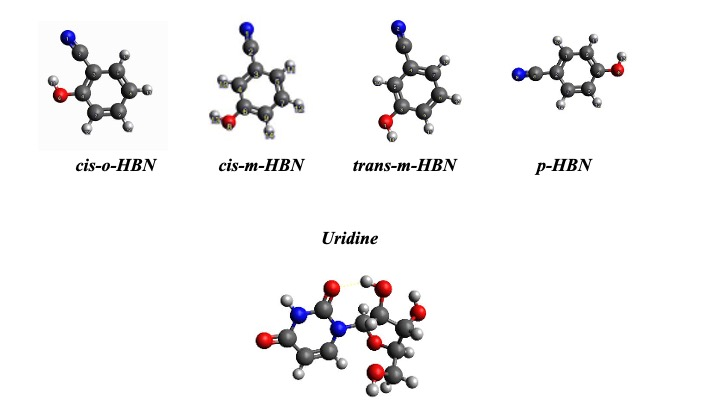
\includegraphics[width=1.0\linewidth]{molecules_CeDiTT.jpg}
\caption{Structures of hydroxybenzonitrile (HBN) isomers and uridine.}
\label{fig:structures}
\end{figure*}

The quantum-chemical data used in this analysis were obtained within
the Pisa Composite Scheme (PCS) framework,\cite{wires_2025,acr_2026}
which has been validated for molecular structures and spectroscopic 
parameters.\cite{BHPCS2_2025,LCB25_2025,pccp_2025}
In particular, equilibrium structures and harmonic force fields were 
computed with the version employing a double-hybrid functional (DPCS3),
while vibrational corrections to rotational constants were obtained with 
the version employing a hybrid functional at (HPCS2). Tensor reconstruction, 
transport, and diagnostic analyses were performed using the CeDiTT program.

For the four HBN isomers (\emph{o}-HBN, \emph{p}-HBN, \emph{cis}-m-HBN,
and \emph{trans}-m-HBN), Table~\ref{table:hbn_main} collects the
ground-state rotational constants and quartic centrifugal distortion
constants in the $I^r$ representation ($A$ reduction), together with
the diagnostic quantity $\log_{10}|s_{111}|$. These are precisely the
quantities typically inspected to assess the numerical stability of a
given representation.

The numerical pattern is clear. In the native $I^r$ ($A$) description,
the quartic constants remain small and chemically well behaved across
the four isomers, and the corresponding $\log_{10}|s_{111}|$ values lie
in the $-10$ to $-11$ range. This is the characteristic signature of a
well-conditioned linear tensor sector.

This behavior contrasts with the strong representation dependence
observed in cases such as DMSO. The HBN family therefore provides a
complementary example in which the standard linear sector remains
robust even for systems of intermediate size.

More generally, the HBN isomers bridge the gap between classical
small-molecule benchmarks and the medium-sized systems that motivate
the present work. The PCS calculations used here are representative of
the level of accuracy that is becoming routinely available for
molecules containing several tens of atoms.

\begin{table*}[t]
\centering
\scriptsize
\setlength{\tabcolsep}{4pt}

\caption{Ground-state rotational constants (MHz) and quartic
centrifugal-distortion constants (kHz) for the four HBN isomers in the
$I^r$ representation ($A$ reduction). Ground-state rotational
constants were obtained by subtracting HPCS2 vibrational corrections
from equilibrium values computed at the DPCS3 level. The diagnostic
parameter $s_{111}$ is reported as $\log_{10}|s_{111}|$.}

\begin{tabular}{lccc ccc ccc ccc}
\toprule
& \multicolumn{3}{c}{\textbf{cis-$o$-HBN}}
& \multicolumn{3}{c}{\textbf{$p$-HBN}}
& \multicolumn{3}{c}{\textbf{cis-$m$-HBN}}
& \multicolumn{3}{c}{\textbf{trans-$m$-HBN}} \\
\cmidrule(lr){2-4}
\cmidrule(lr){5-7}
\cmidrule(lr){8-10}
\cmidrule(lr){11-13}
Parameter
& Exp. & HPCS2 & DPCS3
& Exp. & HPCS2 & DPCS3
& Exp. & HPCS2 & DPCS3
& Exp. & HPCS2 & DPCS3 \\
\midrule

\multicolumn{13}{c}{\textbf{Rotational constants (MHz)}} \\

$B_a$ & 3053.7 & 3037.2 & 3062.1
& 5613.0 & 5596.5 & 5638.8
& 3408.9 & 3398.4 & 3418.6
& 3403.1 & 3390.4 & 3412.8 \\

$B_b$ & 1511.3 & 1506.4 & 1512.6
& 990.5 & 986.5 & 990.7
& 1205.8 & 1201.0 & 1206.6
& 1208.5 & 1204.1 & 1209.2 \\

$B_c$ & 1010.8 & 1006.8 & 1012.3
& 841.9 & 838.7 & 842.7
& 890.7 & 887.3 & 891.8
& 891.8 & 888.4 & 892.9 \\

\midrule
\multicolumn{13}{c}{\textbf{Quartic constants in $I^r$ ($A$ reduction) (kHz)}} \\

$\Delta_J$ & 0.038 & 0.0368 & 0.0370
& 0.020 & 0.015 & 0.016
& 0.041 & 0.0387 & 0.0390
& 0.040 & 0.0380 & 0.0383 \\

$\Delta_{JK}$ & 0.624 & 0.619 & 0.6204
& 0.231 & 0.221 & 0.223
& 0.027 & 0.0246 & 0.0250
& 0.020 & 0.0352 & 0.0356 \\

$\Delta_K$ & -0.100 & 0.381 & 0.384
& 0.900 & 0.918 & 0.922
& 1.180 & 1.173 & 1.178
& 1.130 & 1.158 & 1.161 \\

$\delta_J$ & 0.011 & 0.010 & 0.010
& 0.005 & 0.003 & 0.003
& 0.014 & 0.014 & 0.014
& 0.014 & 0.014 & 0.014 \\

$\delta_K$ & 0.280 & 0.332 & 0.335
& 0.400 & 0.182 & 0.184
& 0.160 & 0.182 & 0.185
& 0.220 & 0.182 & 0.185 \\

$\log_{10}|s_{111}|$ & -10.43 & -10.33 & -10.33
& -11.27 & -11.71 & -11.71
& -11.36 & -11.20 & -11.19
& -11.00 & -11.19 & -11.18 \\

\bottomrule
\end{tabular}

\label{table:hbn_main}
\end{table*}

The HBN example therefore serves two complementary purposes. First, it
shows that the tensor transport machinery remains fully operational
for systems that go beyond traditional small-molecule benchmarks.
Second, it provides a realistic platform for extending the analysis to
the sextic level, where the separation between harmonic, semi-diagonal
cubic, and full cubic contributions becomes both computationally and
physically meaningful.


\subsection{Uridine: a demanding dual-level spectroscopic case}

The present framework can be extended well beyond traditional
benchmark systems. Gas-phase uridine (see Figure~\ref{fig:structures})
provides a demanding test case, combining a 29-atom structure, 
high-resolution experimental data, and a computational setting in 
which a dual-level treatment is both realistic and 
informative.\cite{uridine_2015}

In this work, equilibrium rotational constants were obtained at the
DPCS3 and BDPCS3 levels, while vibrational corrections and centrifugal
distortion constants were computed at the HPCS2 level. This defines a
dual-level strategy (BDPCS3//HPCS2) that is representative of current
computational spectroscopy workflows for medium-sized 
molecules.\cite{acr_2026} Tensor reconstruction and transport were 
performed using CeDiTT.

Table~\ref{tab:uridine_rotational_duallevel} compares experimental
ground-state rotational constants with HPCS2//HPCS2, DPCS3//HPCS2,
and BDPCS3//HPCS2 predictions. Vibrational corrections are clearly
non-negligible, particularly for the largest rotational constant, and
their inclusion is essential for meaningful comparison with
experiment.

The dual-level comparison is selective. The BDPCS3//HPCS2 combination
provides the best agreement, with a mean absolute percentage error of
about $0.20\%$, compared with $0.44\%$ for HPCS2//HPCS2 and $0.53\%$
for DPCS3//HPCS2. This level of accuracy is already notable for a
system of this size and establishes a reliable baseline for the
analysis of centrifugal distortion.

\begin{table*}[t]
\centering
\scriptsize
\caption{Uridine as a demanding dual-level case. Experimental
ground-state rotational constants are from
Ref.~\citenum{uridine_2015}. The notation X//HPCS2 indicates that
equilibrium constants are taken at level X and corrected by HPCS2
vibrational contributions. The last row reports the mean absolute
percentage error (MAE\%) with respect to experiment.}

\begin{tabular}{lcccc}
\hline
Constant & Exp. ($B_0$) & HPCS2//HPCS2 & DPCS3//HPCS2 & BDPCS3//HPCS2 \\
\hline
$A$ (MHz) & 885.98961(14) & 881.93503 & 880.81087 & 883.90684 \\
$B$ (MHz) & 335.59622(35) & 334.44150 & 334.13848 & 335.10385 \\
$C$ (MHz) & 270.11210(20) & 268.70421 & 268.76154 & 269.53137 \\
\hline
MAE (\%) & --- & 0.441 & 0.531 & 0.199 \\
\hline
\end{tabular}
\label{tab:uridine_rotational_duallevel}
\end{table*}

The quartic constants provide further insight. Since the supplied
geometry is already expressed in the $I^r$ representation, the HPCS2
quartic constants can be directly transported to alternative
representations. Table~\ref{tab:uridine_quartic_comparison} reports
the native $I^r$ and transported $III^r$ values.

Only one quartic constant, $D_J = 0.0115(10)$~kHz, was resolved
experimentally. The native $I^r$ prediction ($0.00873$~kHz) lies in
the same range, whereas the transported $III^r$ values show a strong
redistribution of anisotropic contributions.

This behavior is spectroscopically relevant. For a molecule of this
size, a complete quartic fit is typically not feasible, and only a
limited subset of parameters can be determined experimentally. The
tensor framework provides guidance in this situation: in the native
$I^r$ representation, $D_J$, $D_{JK}$, and $D_K$ emerge as the only
quartic terms of significant magnitude and are therefore the most
likely candidates for inclusion in a stable fit.

\begin{table*}[t]
\centering
\scriptsize
\caption{Uridine quartic centrifugal distortion constants from the
HPCS2 vibrational treatment, reported in the native $I^r$
representation and after transport to $III^r$. Only $D_J$ was
resolved experimentally.}

\begin{tabular}{lccc}
\hline
Quantity & Experiment & HPCS2 ($I^r$) & HPCS2 ($III^r$) \\
\hline
$\Delta_J$ (kHz) & --- & 0.010458 & 0.034881 \\
$\Delta_{JK}$ (kHz) & --- & 0.147760 & 0.074491 \\
$\Delta_K$ (kHz) & --- & -0.097394 & -0.097394 \\
$\delta_J$ (kHz) & --- & 0.000760 & -0.012972 \\
$\delta_K$ (kHz) & --- & 0.061064 & -0.050023 \\
\hline
$D_J$ (kHz) & 0.0115(10) & 0.008729 & 0.066718 \\
$D_{JK}$ (kHz) & --- & 0.158135 & -0.116532 \\
$D_K$ (kHz) & --- & -0.106040 & 0.061792 \\
$d_1$ (kHz) & --- & -0.000760 & 0.012972 \\
$d_2$ (kHz) & --- & -0.000865 & 0.015919 \\
\hline
\end{tabular}
\label{tab:uridine_quartic_comparison}
\end{table*}

The contrast between representations is already evident in
Table~\ref{tab:uridine_quartic_comparison}. While the $A$ and $S$
reductions remain mathematically equivalent, they do not provide
equally stable or intuitive parametrizations. The tensor transport
approach resolves this issue by separating intrinsic tensorial
content from representation-dependent effects.

Uridine therefore illustrates a key practical point. For large
molecules, the goal is no longer a complete determination of all
spectroscopic constants, but rather a selective and physically guided
description. In this regime, the tensor framework remains effective:
it supports accurate dual-level rotational constants, enables
representation-consistent transport of quartic parameters, and
provides a rational criterion for identifying the spectroscopically
relevant distortion terms.

This demonstrates that tensor transport remains operational and
spectroscopically useful in the regime where traditional full
parameter determination is no longer feasible.


\subsection{Non-linearity diagnostics}

The standard linear tensor sector does not exhaust the full
perturbative structure of centrifugal distortion. A key practical
question is therefore how to detect its first breakdown in a form that
remains computationally inexpensive and operationally useful. Within
the present framework, this role is played by the quartic channel
$H_{22}$.

Water and formaldehyde provide an instructive comparison. For H$_2$O,
differences between standard VPT-based quartic constants and
higher-level variational results are known to be significant, whereas
for H$_2$CO the same discrepancies are much smaller. The behavior of
the present diagnostic follows the same pattern.

For H$_2$O, the projected contribution $\tau(H_{22})$ is non-negligible
on the scale of the fitted quartic constants and of the VPT--VCI
differences. For H$_2$CO, the same quantity is smaller by roughly two
orders of magnitude. This contrast is precisely what is expected from
a useful first-breakdown indicator: it becomes sizable where the
standard perturbative picture is under strain and remains negligible
where it is already reliable.

The role of $H_{22}$ is therefore not to provide the full correction
beyond the standard quartic sector. Rather, it represents the first
intrinsic tensorial contribution beyond the linear transport picture.
Importantly, it can be evaluated using only quantities already
available in the standard quartic treatment, making it a
computationally inexpensive diagnostic.

In relative terms, $\tau(H_{22})$ corresponds to contributions at the
$10^{-3}$--$10^{-1}$ level of the fitted quartic constants for H$_2$O,
while it becomes negligible for H$_2$CO. This behavior confirms that
$H_{22}$ provides a practical indicator of when the linear tensor
approximation may cease to be quantitatively adequate.

The same logic extends naturally to the sextic sector. Once the
standard sextic geometry functional is expressed in terms of the
quartic tensor, the first post-standard contribution is obtained by
introducing the correction
\begin{equation}
\tau = \tau_{\mathrm{std}} + \tau(H_{22}),
\end{equation}
and retaining the term linear in $\tau(H_{22})$.

This defines a sextic diagnostic that probes how the first
nonlinearity at the quartic level propagates into the sextic problem.

For H$_2$O, the resulting contribution is nonzero and measurable, with
its largest component of the order of $10^3$~Hz. Although much smaller
than the dominant standard sextic constants, this term lies well above
numerical noise and therefore provides a clear signal of the onset of
post-standard effects.

In particular, the largest contribution (about $1.3\times10^3$~Hz)
appears in the $\Phi_{aaa}$ channel and corresponds to a relative
correction of approximately $10^{-3}$ with respect to the dominant
sextic constants. This confirms that the sextic response remains
perturbative, but also shows how the breakdown of the linear quartic
sector propagates into higher-order centrifugal distortion.

The linear response in $\tau(H_{22})$ therefore provides a natural and
computationally inexpensive extension of the quartic diagnostic,
linking the first nonlinear tensorial contribution to the structure of
the sextic geometry sector.


\subsection{Scalability and modern spectroscopic scope}

Modern rotational spectroscopy and quantum-chemical workflows now
routinely address molecules containing several tens of atoms, and the
tensor lifting and transport strategy developed here is fully
compatible with this scale, as it does not introduce additional
tensorial objects beyond those already required for standard
rovibrational treatments. From a computational perspective, the cost 
of tensor reconstruction and transport scales linearly with the number 
of spectroscopic parameters and is negligible compared to the evaluation 
of the underlying force field.

This point is essential for the scope of the present work. The
framework is not only methodological, but provides a practical tool
for organizing fitted and computed centrifugal-distortion constants
in medium-sized systems, identifying numerically stable
representations, and detecting the onset of breakdown of the linear
tensor sector.

This picture is supported by the current availability of accurate
harmonic force fields and partial cubic information for many molecules
of intermediate size. In this regime, low-cost diagnostics become
particularly valuable. The quartic $H_{22}$ contribution introduced
above is of precisely this type, as it can be evaluated using the same
first-order ingredients entering the harmonic model, without requiring
higher-order force constants.

The same logic extends to the sextic sector. The decomposition of the
sextic tensor into geometric, semi-diagonal cubic, and genuine
three-index cubic contributions naturally defines a computational
hierarchy:
\begin{enumerate}
\item geometry (harmonic model),
\item semi-diagonal cubic sector,
\item full three-index cubic contribution.
\end{enumerate}

Within the present tensor formulation, these contributions are
organized without altering the underlying linear tensor mapping, so
that the hierarchy reflects computational complexity rather than the
introduction of new tensorial degrees of freedom.

This hierarchy is not only formal, but reflects actual computational
cost. In finite-difference schemes based on analytic gradients, the
semi-diagonal cubic contribution scales linearly with the number of
vibrational modes, whereas the full three-index cubic sector scales
quadratically.\cite{cubic-vib_2024,pccp_2025}

The numerical examples reported in
Table~\ref{tab:sextic_cubic_hierarchy} illustrate how this hierarchy
is realized in practice. For water, the genuinely three-index cubic
contribution vanishes for all standard sextic components, so that the
full sextic constants are recovered from the geometry and
semi-diagonal cubic sectors alone. For formaldehyde and
thioformaldehyde, the three-index contribution becomes nonzero but
remains subleading in the dominant channels.

In particular, for H$_2$CO the three-index cubic term contributes
only about $3\%$ to the dominant $\Phi_{aaa}$ component, while for
H$_2$CS it drops below $0.1\%$. A similar trend is observed for
F$_2$CO, where the three-index contribution amounts to only
$0.26\%$ of the total.

\begin{table*}[t]
\centering
\caption{Dominant sextic component and decomposition into geometry,
semi-diagonal cubic, and genuine three-index cubic contributions for
four illustrative molecules, all expressed in a common $I^r$
representation. All values are in Hz.}

\begin{tabular}{lcccccc}
\hline
Molecule & Dominant component & Geometry & Cubic 2-index & Cubic 3-index & Total & 3-index / total \\
\hline
H$_2$O  & $\Phi_{aaa}$ & $7.72\times10^5$ & $9.08\times10^4$ & $0$ & $8.62\times10^5$ & $0.0\%$ \\
H$_2$CO & $\Phi_{aaa}$ & $4.11\times10^3$ & $-5.58\times10^2$ & $1.18\times10^2$ & $3.67\times10^3$ & $3.2\%$ \\
H$_2$CS & $\Phi_{aaa}$ & $5.05\times10^3$ & $-3.76\times10^1$ & $3.32$ & $5.02\times10^3$ & $0.07\%$ \\
F$_2$CO & $\Phi_{aaa}$ & $6.67\times10^{-2}$ & $1.19\times10^{-2}$ & $2.07\times10^{-4}$ & $7.88\times10^{-2}$ & $0.26\%$ \\
\hline
\end{tabular}

\label{tab:sextic_cubic_hierarchy}
\end{table*}

Taken together, these results show that the genuinely three-index
cubic sector is not universally negligible, but often remains much
smaller than the geometric and semi-diagonal cubic contributions in
the dominant sextic channels.

This observation has direct practical implications. It suggests that,
for many medium-sized systems, a reduced computational strategy based
on harmonic information and semi-diagonal cubic terms may already
capture the leading sextic behavior, while the full cubic treatment
can be reserved for cases where higher accuracy is required.

The tensor framework provides the natural setting for exploiting this
hierarchy, allowing different levels of approximation to be combined
consistently within a single representation-independent description.


\section{Conclusions}

In this work, a tensorial framework for the analysis and transport of
centrifugal distortion constants has been introduced. The central
result is that conventional quartic and standard sextic constants can
be consistently interpreted within a common tensorial sector generated
by combinations of the first derivatives of the inverse inertia tensor.
Within this formulation, Watson parameters are recognized as
representation-dependent projections of underlying tensor
representatives, so that different Hamiltonian reductions and axis
representations correspond to alternative parametrizations of the same
rovibrational structure.

This perspective clarifies the origin of the strong representation
dependence of centrifugal-distortion parameters and shows that, within
the standard sector, no additional independent tensorial degrees of
freedom are introduced at the sextic level in the mapping to
spectroscopic parameters. Importantly, the linearity refers to the
mapping between tensor representatives and spectroscopic parameters,
which remains linear even when anharmonic contributions from cubic
force constants are included. These contributions extend the physical
content of the model without altering the tensorial structure of the
mapping.

The first intrinsic breakdown of this linear regime is identified at
quartic order through the $H_{22}$ contribution, which introduces a
second-level geometric tensor beyond the $\mu_1$-generated sector. This
contribution propagates into the sextic level through a corresponding
linear response, defining a natural hierarchy of tensorial corrections
beyond the standard perturbative framework.

A key feature of the present approach is its operational character.
Tensor representatives are reconstructed from spectroscopic parameters
through SVD-based pseudoinverse techniques, providing a stable and
well-defined solution of the inverse problem. This construction selects
the minimum-norm tensor compatible with the data and corresponds to the
least-structured tensor consistent with the input, thereby avoiding
spurious contributions in the null space of the projection operator.
The resulting lift--transport--reprojection procedure enables
consistent and robust transformations between representations.

The formulation also leads to simple and computationally inexpensive
diagnostics, such as the $H_{22}$ indicator and its sextic analogue,
which quantify the onset of deviations from the linear tensor regime
and provide predictive information on the sensitivity of centrifugal
distortion constants to Hamiltonian representation.

The methodology is implemented in the CeDiTT program and is applicable
to both experimental and quantum-chemical datasets. In this way,
centrifugal-distortion constants can be analyzed, compared, and
transported within a unified and representation-independent framework.

Beyond methodological aspects, the present results demonstrate that the
tensor formulation remains effective for medium- and large-sized
molecular systems. Combined with modern computational workflows, it
provides a practical route for scalable and physically grounded
analysis of centrifugal distortion, while offering a natural basis for
future extensions toward higher-order treatments and data-driven
approaches.

Overall, the present work establishes a unified and scalable framework
in which representation-dependent spectroscopic parameters are recast
as projections of underlying tensorial objects, providing both a
conceptual clarification and a practical tool for modern rotational
spectroscopy.


\section{Appendix}

The appendices are organized as follows.

Appendix~A presents the reconstruction of the quartic tensor,
including its projection onto Watson constants and the associated
pseudoinverse gauge fixing.

Appendix~B gives the explicit partition of the standard sextic tensor
into geometry, semi-diagonal cubic, and genuine three-index cubic
sectors.

Appendix~C describes the projection of the sextic tensor onto the usual
spectroscopic constants.

Appendix~D discusses the limiting cases of symmetric tops, spherical
tops, and linear molecules, where symmetry-adapted projections are
required.

Appendix~E summarizes the computational procedures used to implement
the tensor transport machinery and its current operational extensions.


\section{Appendix A: Quartic Tensor Reconstruction and Pseudoinverse Gauge Fixing}

The quartic centrifugal–distortion sector is conveniently described
in terms of the pair–pair quartic tensor

\begin{equation}
\boldsymbol{\tau}^{(4)} =
\bigl(
\tau_{aaaa},\tau_{bbbb},\tau_{cccc},
\tau_{aabb},\tau_{aacc},\tau_{bbcc}
\bigr)^T ,
\end{equation}

or, equivalently, through the reduced symmetric matrix

\begin{equation}
\tau'=
\begin{pmatrix}
\tau_{aaaa} & \tau_{aabb}/2 & \tau_{aacc}/2 \\
\tau_{aabb}/2 & \tau_{bbbb} & \tau_{bbcc}/2 \\
\tau_{aacc}/2 & \tau_{bbcc}/2 & \tau_{cccc}
\end{pmatrix}.
\end{equation}

This representation contains six independent components and provides
a compact basis for tensor transport.

Once $\tau'$ is reconstructed, one defines

\begin{equation}
T_{ij} = \frac{\tau'_{ij}}{4}.
\end{equation}

From these quantities the cylindrical combinations are constructed:

\begin{align}
T_{400} &= \frac{3T_{aa}+3T_{bb}+2T_{ab}}{8}, \\
T_{220} &= T_{ac}+T_{bc}-2T_{400}, \\
T_{040} &= T_{cc}-T_{220}-T_{400}, \\
T_{202} &= \frac{T_{aa}-T_{bb}}{4}, \\
T_{022} &= \frac{T_{ac}-T_{bc}}{2}-T_{202}, \\
T_{004} &= \frac{T_{aa}+T_{bb}-2T_{ab}}{16}.
\end{align}

\subsection{Projection to Watson constants}

The mapping from tensor space to spectroscopic parameters is linear.
For Watson’s $A$ reduction one has

\begin{align}
\Delta_J   &= -T_{400}-2T_{004}, \\
\Delta_{JK}&= -T_{220}+12T_{004}, \\
\Delta_K   &= -T_{040}-10T_{004}, \\
\delta_J   &= -T_{202}, \\
\delta_K   &= -T_{022}-4\Sigma T_{004},
\end{align}

with

\begin{equation}
\Sigma = \frac{2A-B-C}{B-C}.
\end{equation}

For the $S$ reduction,

\begin{align}
D_J   &= -T_{400}+\frac12 T_{022}\Sigma_1, \\
D_{JK}&= -T_{220}-3T_{022}\Sigma_1, \\
D_K   &= -T_{040}+\frac52 T_{022}\Sigma_1, \\
d_1   &= T_{202}, \\
d_2   &= T_{004}+\frac14 T_{022}\Sigma_1,
\end{align}

with

\begin{equation}
\Sigma_1 = \frac{B-C}{2A-B-C} = \Sigma^{-1}.
\end{equation}

\subsection{Rank deficiency and reduction-independent null sector}

The projection from the six-dimensional tensor space to the five
quartic spectroscopic constants defines a linear map

\begin{equation}
\mathbf W = \mathbf P\, \mathbf T,
\end{equation}

where $\mathbf T \in \mathbb{R}^6$ and $\mathbf W \in \mathbb{R}^5$.
Since $\mathrm{rank}(\mathbf P)=5$, the kernel of $\mathbf P$ is
one-dimensional.

The $A$ and $S$ reductions correspond to two linear projections
$\mathbf P^{(A)}$ and $\mathbf P^{(S)}$ related by an invertible
transformation in parameter space,

\begin{equation}
\mathbf W^{(S)} = \mathbf M \, \mathbf W^{(A)},
\qquad
\mathbf M \in \mathrm{GL}(5).
\end{equation}

It follows that

\begin{equation}
\mathbf P^{(S)} = \mathbf M \mathbf P^{(A)},
\end{equation}

and therefore

\begin{equation}
\ker(\mathbf P^{(S)}) = \ker(\mathbf P^{(A)}).
\end{equation}

The null space is thus a structural property of the projection from
tensor space to spectroscopic parameters and is independent of the
chosen Watson reduction.

A representative null vector can be obtained by solving
$\mathbf P^{(A)} \mathbf n = 0$, yielding

\begin{equation}
\mathbf n =
\left(
0,\,
0,\,
0,\,
1,\,
\frac{\Sigma-1}{2},\,
-\frac{\Sigma+1}{2}
\right)^T .
\end{equation}

In matrix form this corresponds to the null tensor

\begin{equation}
N'=
\begin{pmatrix}
0 & 1/2 & (\Sigma-1)/4 \\
1/2 & 0 & -(\Sigma+1)/4 \\
(\Sigma-1)/4 & -(\Sigma+1)/4 & 0
\end{pmatrix}.
\end{equation}

If $\tau'$ reproduces a given set of quartic spectroscopic constants,
then

\begin{equation}
\tau' + \eta N'
\end{equation}

reproduces the same constants for any $\eta \in \mathbb{R}$,
independently of the chosen reduction.

\subsection{Pseudoinverse gauge fixing}

To remove this affine indeterminacy, the Moore–Penrose pseudoinverse
is used to select the minimum-norm solution of the inverse problem,

\begin{equation}
\mathbf T = \mathbf P^{+} \mathbf W.
\end{equation}

This choice defines a linear gauge condition that selects a unique
representative within the affine family,

\begin{equation}
2\tau'_{ab}+(\Sigma-1)\tau'_{ac}-(\Sigma+1)\tau'_{bc}=0.
\label{eq:app_quartic_gauge}
\end{equation}

This condition does not represent a physical constraint, but the
orthogonality condition that defines the Moore–Penrose solution,
i.e. the reconstructed tensor is orthogonal to the null space of the
projection operator.

The existence of this gauge reflects the fact that Watson
parametrizations do not span the full tensor space, and that the
inverse problem admits infinitely many solutions differing by
components in the null direction.

The null vector can be interpreted as the unique direction in tensor
space that does not couple to any quartic rotational operator.


\section{Appendix B: Explicit Partition of the Standard Sextic Tensor}

\subsection{Explicit standard sextic partition}

The standard sextic Cartesian components are built in the principal-axis frame.
In this subsection the vibrational indices are denoted by $i,j,k,\ldots$,
whereas $a,b,c$ denote principal-axis labels. The reduced cubic force constants
$\Phi^{(3),\mathrm{red}}_{ijk}$ are the fully symmetrized Gaussian normal-mode
constants reordered into the working vibrational basis.

To expose the harmonic scaling, define
\begin{equation}
\widetilde{\mu}^{(i)}_{ab}
=
-\frac{(I_0\,\mu^{(i)}\,I_0)_{ab}}
{2\,M_a M_b\,\kappa_i},
\qquad
\kappa_i
=
\mathrm{DIDQ}_0\,(\mathrm{FACTG}\,\omega_i)^{3/2},
\end{equation}
and the rescaled first-level tensor
\begin{equation}
\mathcal{M}^{(i)}_{ab}
=
\omega_i^{3/2}\widetilde{\mu}^{(i)}_{ab}.
\end{equation}
The quartic tensor then reads
\begin{equation}
\tau_{abcd}
=
-2\sum_i
\frac{\mathcal{M}^{(i)}_{ab}\mathcal{M}^{(i)}_{cd}}{\omega_i^2},
\label{eq:app_sextic_tau_from_mu1}
\end{equation}
so that each quartic insertion carries explicitly the standard harmonic
denominator $\omega_i^{-2}$.

The Coriolis-dressed first-level quantity entering the sextic geometry sector
is
\begin{equation}
\widetilde{\nu}^{(i)}_{abc}
=
\sum_j
\frac{2}{3}\,
\frac{\omega_i^2+2\omega_j^2}{\omega_i^{5/2}\omega_j^2}
\Big[
B_a\,\zeta^{(a)}_{ij}\,\mathcal{M}^{(j)}_{bc}
+
B_b\,\zeta^{(b)}_{ij}\,\mathcal{M}^{(j)}_{ca}
+
B_c\,\zeta^{(c)}_{ij}\,\mathcal{M}^{(j)}_{ab}
\Big].
\label{eq:app_sextic_nu_from_mu1}
\end{equation}
All sextic contributions built only from $\tau$ and $\widetilde{\nu}$ are
therefore homogeneous of order $\omega^{-4}$, whereas the explicit cubic
contributions are homogeneous of order $\omega^{-3}$.

\paragraph{Diagonal class $\Phi_{aaa}$.}
For a repeated principal axis $a$ one has
\begin{equation}
\Phi_{aaa}=X_1-X_2+X_3+X_4,
\end{equation}
with
\begin{align}
X_1 &= \frac{3}{16}\sum_x\frac{\tau_{aaax}^2}{B_x},&
X_2 &= \frac{1}{2}\sum_i \omega_i\left(\widetilde{\nu}^{(i)}_{aaa}\right)^2,\\
X_3 &= \frac{1}{6}\sum_{i,j,k}
\frac{\Phi^{(3),\mathrm{red}}_{ijk}}{\omega_i\omega_j\omega_k}\,
\mathcal{M}^{(i)}_{aa}\mathcal{M}^{(j)}_{aa}\mathcal{M}^{(k)}_{aa},&
X_4 &= \frac{1}{4}\sum_{x\neq a}
\frac{\tau_{xaaa}^2}{B_a-B_x}.
\end{align}
The cubic term is partitioned as
\begin{equation}
X_3=X_3^{(2)}+X_3^{(3)},
\end{equation}
where
\begin{align}
X_3^{(2)}
&=
\frac{1}{6}\sum_i
\frac{\Phi^{(3),\mathrm{red}}_{iii}}{\omega_i^3}
\left(\mathcal{M}^{(i)}_{aa}\right)^3
+\frac{1}{2}\sum_{i\neq j}
\frac{\Phi^{(3),\mathrm{red}}_{iij}}{\omega_i^2\omega_j}
\left(\mathcal{M}^{(i)}_{aa}\right)^2\mathcal{M}^{(j)}_{aa},
\\
X_3^{(3)}
&=
\sum_{i<j<k}
\frac{\Phi^{(3),\mathrm{red}}_{ijk}}{\omega_i\omega_j\omega_k}
\mathcal{M}^{(i)}_{aa}\mathcal{M}^{(j)}_{aa}\mathcal{M}^{(k)}_{aa}.
\end{align}

\paragraph{Mixed class $\Phi_{aab}$.}
For $a\neq b$ one obtains
\begin{equation}
\Phi_{aab}=Y_1-Y_2+Y_3+Y_4+Y_5+Y_6,
\end{equation}
with
\begin{align}
Y_1 &=
\frac{3}{32}\sum_x
\frac{T_{abx}^2+2\tau_{aaax}U_{abx}}{B_x},&
T_{abx} &= \tau_{aabx}+2\tau_{abax},&
U_{abx} &= \tau_{bbax}+2\tau_{abbx},\\
Y_2 &=
\frac{3}{4}\sum_i \omega_i
\left[
3\left(\widetilde{\nu}^{(i)}_{aab}\right)^2
+2\,\widetilde{\nu}^{(i)}_{aaa}\widetilde{\nu}^{(i)}_{abb}
\right],\\
Y_3 &=
\frac{1}{4}\sum_{i,j,k}
\frac{\Phi^{(3),\mathrm{red}}_{ijk}}{\omega_i\omega_j\omega_k}
\mathcal{M}^{(k)}_{aa}
\left[
\mathcal{M}^{(i)}_{aa}\mathcal{M}^{(j)}_{bb}
+4\mathcal{M}^{(i)}_{ab}\mathcal{M}^{(j)}_{ab}
\right],\\
Y_4 &=
\frac{\tau_{aaab}\left(4\tau_{bbba}-3\tau_{aaab}\right)}
{8(B_a-B_b)},\\
Y_5 &=
\sum_{x\neq a,b}
\frac{
\tau_{aaax}
\Big[
(B_a-B_x)(\tau_{bbax}+2\tau_{babx})
+(B_a-B_b)(\tau_{xxxa}-\tau_{aaax})
\Big]}
{4(B_a-B_x)^2},\\
Y_6 &=
\sum_{x\neq a,b}
\frac{
(\tau_{aabx}+2\tau_{abax})
\Big[
(B_b-B_x)(\tau_{aabx}+2\tau_{abax})
+2(B_a-B_b)(\tau_{bbbx}-\tau_{xxxb})
\Big]}
{8(B_b-B_x)^2}.
\end{align}
The cubic term is
\begin{equation}
Y_3=Y_3^{(2)}+Y_3^{(3)},
\end{equation}
with
\begin{align}
Y_3^{(2)}
&=
\frac{1}{4}\sum_i
\frac{\Phi^{(3),\mathrm{red}}_{iii}}{\omega_i^3}
\mathcal{M}^{(i)}_{aa}
\left[
\mathcal{M}^{(i)}_{aa}\mathcal{M}^{(i)}_{bb}
+4\left(\mathcal{M}^{(i)}_{ab}\right)^2
\right]
\notag\\
&\quad
+\frac{1}{4}\sum_{i\neq j}
\frac{\Phi^{(3),\mathrm{red}}_{iij}}{\omega_i^2\omega_j}
\Big\{
\mathcal{M}^{(j)}_{aa}
\left[
\mathcal{M}^{(i)}_{aa}\mathcal{M}^{(i)}_{bb}
+4\left(\mathcal{M}^{(i)}_{ab}\right)^2
\right]
\notag\\
&\qquad\qquad
+\mathcal{M}^{(i)}_{aa}
\left[
\mathcal{M}^{(i)}_{aa}\mathcal{M}^{(j)}_{bb}
+4\mathcal{M}^{(i)}_{ab}\mathcal{M}^{(j)}_{ab}
\right]
\notag\\
&\qquad\qquad
+\mathcal{M}^{(i)}_{aa}
\left[
\mathcal{M}^{(j)}_{aa}\mathcal{M}^{(i)}_{bb}
+4\mathcal{M}^{(j)}_{ab}\mathcal{M}^{(i)}_{ab}
\right]
\Big\},
\\
Y_3^{(3)}
&=
\frac{1}{4}\sum_{i<j<k}
\frac{\Phi^{(3),\mathrm{red}}_{ijk}}{\omega_i\omega_j\omega_k}
\sum_{\pi\in S_3}
\mathcal{M}^{(\pi_3)}_{aa}
\left[
\mathcal{M}^{(\pi_1)}_{aa}\mathcal{M}^{(\pi_2)}_{bb}
+4\mathcal{M}^{(\pi_1)}_{ab}\mathcal{M}^{(\pi_2)}_{ab}
\right].
\end{align}

\paragraph{Fully mixed class $\Phi_{abc}$.}
For three distinct principal axes one has
\begin{equation}
\Phi_{abc}=Z_1-Z_2+Z_3+Z_4,
\end{equation}
with
\begin{align}
Z_1
&=
\frac{3}{16}\sum_x
\frac{
2V_x^2
+W_x^{(ab)}W_x^{(ac)}
+W_x^{(bc)}W_x^{(ba)}
+W_x^{(ca)}W_x^{(cb)}
}{B_x},
\\
V_x &= \tau_{xabc}+\tau_{xbca}+\tau_{xcab},
\\
W_x^{(ab)} &= \tau_{xabb}+2\tau_{xbab},
\qquad
W_x^{(ac)} = \tau_{xacc}+2\tau_{xcac},
\\
W_x^{(bc)} &= \tau_{xbcc}+2\tau_{xcbc},
\qquad
W_x^{(ba)} = \tau_{xbaa}+2\tau_{xaba},
\\
W_x^{(ca)} &= \tau_{xcaa}+2\tau_{xaca},
\qquad
W_x^{(cb)} = \tau_{xcbb}+2\tau_{xbcb},
\\
Z_2
&=
\frac{9}{2}\sum_i\omega_i
\Big[
2\left(\widetilde{\nu}^{(i)}_{abc}\right)^2
+\widetilde{\nu}^{(i)}_{bba}\widetilde{\nu}^{(i)}_{cca}
+\widetilde{\nu}^{(i)}_{ccb}\widetilde{\nu}^{(i)}_{aab}
+\widetilde{\nu}^{(i)}_{aac}\widetilde{\nu}^{(i)}_{bbc}
\Big],
\\
Z_3
&=
\frac{1}{2}\sum_{i,j,k}
\frac{\Phi^{(3),\mathrm{red}}_{ijk}}{\omega_i\omega_j\omega_k}
\Big[
\mathcal{M}^{(i)}_{aa}\mathcal{M}^{(j)}_{bb}\mathcal{M}^{(k)}_{cc}
+2\mathcal{M}^{(i)}_{aa}\mathcal{M}^{(j)}_{bc}\mathcal{M}^{(k)}_{bc}
\notag\\
&\qquad\qquad
+2\mathcal{M}^{(i)}_{bb}\mathcal{M}^{(j)}_{ca}\mathcal{M}^{(k)}_{ca}
+2\mathcal{M}^{(i)}_{cc}\mathcal{M}^{(j)}_{ab}\mathcal{M}^{(k)}_{ab}
+8\mathcal{M}^{(i)}_{bc}\mathcal{M}^{(j)}_{ca}\mathcal{M}^{(k)}_{ab}
\Big],
\\
Z_4
&=
\frac{3}{2}
\sum_{x,y,z\ \mathrm{pairwise\ distinct}}
\frac{
(\tau_{yyyz}-\tau_{zzzy})
\big[(B_z-B_x)\tau_{yyyz}+(B_x-B_y)\tau_{zzzy}\big]
}
{4(B_y-B_z)^2}.
\end{align}
The cubic term is
\begin{equation}
Z_3=Z_3^{(2)}+Z_3^{(3)},
\end{equation}
where
\begin{align}
\mathcal{K}_{abc}(p,q,r)
&=
\mathcal{M}^{(p)}_{aa}\mathcal{M}^{(q)}_{bb}\mathcal{M}^{(r)}_{cc}
+2\mathcal{M}^{(p)}_{aa}\mathcal{M}^{(q)}_{bc}\mathcal{M}^{(r)}_{bc}
\notag\\
&\quad
+2\mathcal{M}^{(p)}_{bb}\mathcal{M}^{(q)}_{ca}\mathcal{M}^{(r)}_{ca}
+2\mathcal{M}^{(p)}_{cc}\mathcal{M}^{(q)}_{ab}\mathcal{M}^{(r)}_{ab}
+8\mathcal{M}^{(p)}_{bc}\mathcal{M}^{(q)}_{ca}\mathcal{M}^{(r)}_{ab},
\\
Z_3^{(2)}
&=
\frac{1}{2}\sum_i
\frac{\Phi^{(3),\mathrm{red}}_{iii}}{\omega_i^3}
\mathcal{K}_{abc}(i,i,i)
\notag\\
&\quad
+\frac{1}{2}\sum_{i\neq j}
\frac{\Phi^{(3),\mathrm{red}}_{iij}}{\omega_i^2\omega_j}
\sum_{\pi\in\{(i,i,j),(i,j,i),(j,i,i)\}}
\mathcal{K}_{abc}(\pi_1,\pi_2,\pi_3),
\\
Z_3^{(3)}
&=
\frac{1}{2}\sum_{i<j<k}
\frac{\Phi^{(3),\mathrm{red}}_{ijk}}{\omega_i\omega_j\omega_k}
\sum_{\pi\in S_3}
\mathcal{K}_{abc}(\pi_1,\pi_2,\pi_3).
\end{align}

Equations~\eqref{eq:app_sextic_tau_from_mu1}--\eqref{eq:app_sextic_nu_from_mu1}
and the componentwise partitions above make the standard hierarchy explicit:
the geometry sector is homogeneous of order $\omega^{-4}$, whereas the cubic
sector is homogeneous of order $\omega^{-3}$.



\section{Appendix C: Sextic Tensor Reconstruction and Projection}

The sextic centrifugal–distortion sector is described in terms of the
Cartesian tensor components in the principal-axis frame,

\[
\Phi_{aaa},\Phi_{aab},\Phi_{aac},\Phi_{abb},\Phi_{abc},\Phi_{acc},
\Phi_{bbb},\Phi_{bbc},\Phi_{bcc},\Phi_{ccc}.
\]

These components are first transformed into cylindrical sextic
quantities, which provide a convenient intermediate representation
for the projection onto spectroscopic parameters:

\begin{align}
\Phi_{600} &= \frac{5}{16}(\Phi_{aaa}+\Phi_{bbb})
+\frac{1}{8}(\Phi_{aab}+\Phi_{abb}),\\
\Phi_{420} &= \frac{3}{4}(\Phi_{aac}+\Phi_{bbc})
+\frac{1}{4}\Phi_{abc}-3\Phi_{600},\\
\Phi_{240} &= \Phi_{acc}+\Phi_{bcc}-2\Phi_{420}-3\Phi_{600},\\
\Phi_{060} &= \Phi_{ccc}-\Phi_{240}-\Phi_{420}-\Phi_{600},\\
\Phi_{402} &= \frac{15}{64}(\Phi_{aaa}-\Phi_{bbb})
+\frac{1}{32}(\Phi_{aab}-\Phi_{abb}),\\
\Phi_{222} &= \frac{1}{2}(\Phi_{aac}-\Phi_{bbc})-2\Phi_{402},\\
\Phi_{042} &= \frac{1}{2}(\Phi_{acc}-\Phi_{bcc})
-\Phi_{222}-\Phi_{402},\\
\Phi_{204} &= \frac{3}{32}(\Phi_{aaa}+\Phi_{bbb})
-\frac{1}{16}(\Phi_{aab}+\Phi_{abb}),\\
\Phi_{024} &= \frac{1}{8}(\Phi_{aac}+\Phi_{bbc}-\Phi_{abc})
-\Phi_{204},\\
\Phi_{006} &= \frac{1}{64}(\Phi_{aaa}-\Phi_{bbb})
-\frac{1}{32}(\Phi_{aab}-\Phi_{abb}).
\end{align}

\subsection{Coupling with the quartic sector}

In contrast to the quartic case, the sextic projection depends not only
on sextic tensor components, but also on quadratic combinations of the
quartic tensor. These contributions arise from the perturbative
structure of the effective Hamiltonian and are expressed through

\begin{align}
B_{200} &= \frac{1}{2}(A+B)-4T_{004},\\
B_{020} &= C-B_{200}+6T_{004},\\
B_{002} &= \frac{1}{4}(A-B),
\end{align}

where the $T_{ijk}$ coefficients are defined from the quartic tensor
as in Appendix~A.

\subsection{Projection to Watson constants: $A$ reduction}

For the $A$ reduction, the sextic centrifugal–distortion constants are

\begin{align}
\Phi_J &= \Phi_{600}+2\Phi_{204},\\
\Phi_{JK} &=
\Phi_{420}-12\Phi_{204}+2\Phi_{024}
+16\Sigma\Phi_{006} \\
&\quad +8\frac{T_{022}\,T_{004}}{B_{002}},\\
\Phi_{KJ} &= \Phi_{240}+\frac{10}{3}\Phi_{420}
-30\Phi_{204}-\frac{10}{3}\Phi_{JK},\\
\Phi_K &= \Phi_{060}-\frac{7}{3}\Phi_{420}
+28\Phi_{204}+\frac{7}{3}\Phi_{JK},\\
\phi_J &= \Phi_{402}+\Phi_{006},\\
\phi_K &=
\Phi_{042}+\frac{4}{3}\Sigma\Phi_{024}
+\left(\frac{32}{3}\Sigma^2+9\right)\Phi_{006} \\
&\quad +4\frac{T_{040}+\frac{1}{3}\Sigma T_{022}
-2(\Sigma^2-2)T_{004}}{B_{002}}T_{004},\\
\phi_{JK} &=
\Phi_{222}+4\Sigma\Phi_{204}-10\Phi_{006} \\
&\quad +2\frac{T_{220}-2\Sigma T_{202}-4T_{004}}{B_{002}}T_{004},
\end{align}

with

\begin{equation}
\Sigma=\frac{2A-B-C}{B-C}.
\end{equation}

\subsection{Projection to Watson constants: $S$ reduction}

For the $S$ reduction, define

\begin{align}
\rho &= \frac{1}{4}T_{022}\Sigma_1,\\
\mu &=
\frac{\Sigma\Phi_{042}-\frac{9}{8}\Phi_{024}}%
{2\Sigma^2+\frac{27}{16}} \\
&\quad +\frac{\bigl(-2\Sigma T_{040}+(\Sigma^2+3)T_{022}
-5\Sigma T_{004}\bigr)T_{022}}%
{B_{020}\left(2\Sigma^2+\frac{27}{16}\right)},\\
\nu &= \frac{3}{16}\mu\Sigma_1+\frac{1}{8}\Phi_{024}\Sigma_1
+\frac{T_{004}\,T_{022}}{B_{020}},\\
\lambda &=
5\nu\Sigma_1+\frac{1}{2}\Phi_{222}\Sigma_1 \\
&\quad +\frac{-\frac{1}{2}T_{220}\Sigma_1+T_{202}
-T_{022}\Sigma_1^2-2T_{004}\Sigma_1}{B_{020}}T_{022},
\end{align}

with

\begin{equation}
\Sigma_1=\frac{B-C}{2A-B-C}.
\end{equation}

The sextic constants are

\begin{align}
H_J &= \Phi_{600}-\lambda,\\
H_{JK} &= \Phi_{420}+6\lambda-3\mu,\\
H_{KJ} &= \Phi_{240}-5\lambda+10\mu,\\
H_K &= \Phi_{060}-7\mu,\\
h_1 &= \Phi_{402}-\nu,\\
h_2 &= \Phi_{204}+\frac{1}{2}\lambda,\\
h_3 &= \Phi_{006}+\nu.
\end{align}

\subsection{Inverse problem and pseudoinverse reconstruction}

The mapping from sextic tensor space to Watson sextic constants is
linear but not invertible, as in the quartic case. Consequently, the
inverse problem admits an affine family of solutions.

The tensor reconstruction is therefore performed using the
Moore–Penrose pseudoinverse, which selects the minimum-norm tensor
compatible with the available spectroscopic parameters. This ensures
consistency with the gauge-fixing procedure adopted for the quartic
tensor and provides a unique tensor representative for the sextic
sector.


\section{Appendix D: Special Limits: Symmetric Tops, Spherical Tops, and Linear Molecules}
\label{sec:appendix_special_limits}

The projection formulas used throughout the main text are written for
nondegenerate asymmetric tops. This is already evident in the quartic
asymmetric-top projection, where the coefficients depend on

\begin{equation}
\Sigma = \frac{2A-B-C}{B-C},
\qquad
\Sigma_1 = \frac{B-C}{2A-B-C}.
\end{equation}

At exact axial symmetry ($B=C$ for a prolate top or $A=B$ for an oblate
top) these expressions become singular. This singularity does not
reflect a failure of the tensorial formulation itself; it only indicates
that the asymmetric-top projection basis is no longer adapted to the
symmetry of the problem. The appropriate treatment is therefore to keep
the tensorial construction unchanged and to replace the final
spectroscopic projection by a symmetry-adapted one.

More generally, the spectroscopic parametrization should not be viewed
as a single coordinate chart that can be smoothly continued across all
rotor classes. Passing from a nondegenerate asymmetric top to an exact
symmetric top changes the isotropy of the inertia tensor and makes the
asymmetric-top projection singular. The spherical-top limit increases
the degeneracy further, while the linear-molecule limit changes the rank
of the inertia tensor itself. What remains common across these cases is
the tensorial hierarchy introduced in the main text; what changes is the
operator basis onto which this tensorial content is projected. The
correct continuity statement is therefore not that the same fitted
constants survive in the limit, but that the same tensorial objects
admit different symmetry-adapted spectroscopic readouts in the different
rotor classes.

\subsection{Symmetric tops}

Let $\mathbf u$ denote the unit vector along the symmetry axis and
define the axial projectors

\begin{equation}
P_{\parallel} = \mathbf u\mathbf u^T,
\qquad
P_{\perp} = \mathbf 1 - P_{\parallel}.
\end{equation}

At equilibrium the inverse inertia tensor can then be written as

\begin{equation}
I^{-1} = \mu_{\parallel} P_{\parallel} + \mu_{\perp} P_{\perp}.
\end{equation}

The first-level tensor $\mu_1=\partial I^{-1}/\partial Q$ and all
derived quantities ($\tau$, $B(\mu_1)$, $N$, $\mu_2$) remain defined
exactly as in the asymmetric-top case. What changes is only the final
projection onto effective-Hamiltonian parameters.

For the quartic sector the natural axial decomposition is

\begin{equation}
\begin{aligned}
\tau_{\alpha\beta\gamma\delta}
&=
4T_{\perp\perp}
P_{\perp,\alpha\beta}P_{\perp,\gamma\delta}
\\
&\quad
+4T_{\perp\parallel}
\left(
P_{\perp,\alpha\beta}P_{\parallel,\gamma\delta}
+
P_{\parallel,\alpha\beta}P_{\perp,\gamma\delta}
\right)
\\
&\quad
+4T_{\parallel\parallel}
P_{\parallel,\alpha\beta}P_{\parallel,\gamma\delta}.
\end{aligned}
\label{eq:app_sym_tau_decomp}
\end{equation}

In operator form this gives

\begin{equation}
H_{\mathrm{cd}}^{(4),\mathrm{sym}}
=
-T_{\perp\perp} (J_{\perp}^2)^2
-T_{\perp\parallel} J_{\perp}^2 J_{\parallel}^2
-T_{\parallel\parallel} J_{\parallel}^4,
\label{eq:app_sym_quartic_operator}
\end{equation}

where

\begin{equation}
J_{\parallel} = \mathbf J\!\cdot\!\mathbf u,
\qquad
J_{\perp}^2 = J^2 - J_{\parallel}^2 .
\end{equation}

Matching Eq.~\eqref{eq:app_sym_quartic_operator} with the standard
symmetric-top quartic Hamiltonian

\begin{equation}
H_{\mathrm{cd}}^{(4),\mathrm{sym}}
=
-D_J J^4
-D_{JK} J^2 J_{\parallel}^2
-D_K J_{\parallel}^4
\end{equation}

yields

\begin{align}
D_J &= T_{\perp\perp}, \\
D_{JK} &= T_{\perp\parallel}-2T_{\perp\perp}, \\
D_K &= T_{\parallel\parallel}-T_{\perp\parallel}+T_{\perp\perp}.
\label{eq:app_sym_quartic_constants}
\end{align}

The asymmetric-top constants $\delta_J$ and $\delta_K$ vanish at exact
axial symmetry because they correspond to anisotropic splitting inside
the degenerate transverse plane.

The same reasoning applies to the sextic sector. The axial operator
basis becomes

\begin{equation}
H_{\mathrm{cd}}^{(6),\mathrm{sym}}
=
-X_0 (J_{\perp}^2)^3
-X_1 (J_{\perp}^2)^2 J_{\parallel}^2
-X_2 J_{\perp}^2 J_{\parallel}^4
-X_3 J_{\parallel}^6 ,
\label{eq:app_sym_sextic_operator}
\end{equation}

which is matched to the usual symmetric-top sextic Hamiltonian

\begin{equation}
H_{\mathrm{cd}}^{(6),\mathrm{sym}}
=
-H_J J^6
-H_{JK} J^4 J_{\parallel}^2
-H_{KJ} J^2 J_{\parallel}^4
-H_K J_{\parallel}^6 .
\end{equation}

Using the identities

\begin{align}
J^6 &= (J_{\perp}^2)^3 +3(J_{\perp}^2)^2J_{\parallel}^2
+3J_{\perp}^2J_{\parallel}^4 +J_{\parallel}^6, \\
J^4J_{\parallel}^2 &= (J_{\perp}^2)^2J_{\parallel}^2
+2J_{\perp}^2J_{\parallel}^4 +J_{\parallel}^6, \\
J^2J_{\parallel}^4 &= J_{\perp}^2J_{\parallel}^4+J_{\parallel}^6 ,
\end{align}

one obtains

\begin{align}
H_J &= X_0, \\
H_{JK} &= X_1-3X_0, \\
H_{KJ} &= X_2-2X_1+3X_0, \\
H_K &= X_3-X_2+X_1-X_0 .
\label{eq:app_sym_sextic_constants}
\end{align}

Operationally the tensorial sextic construction and the linear response
in $\tau(H_{22})$ are evaluated exactly as in the asymmetric-top case
and then projected onto the axial coefficients $X_0,\ldots,X_3$ rather
than onto asymmetric-top Watson constants.

\subsection{Spherical tops}

For a spherical top the equilibrium inertia tensor is proportional to
the identity,

\begin{equation}
I = I_0 \mathbf 1,
\qquad
I^{-1} = \mu_0 \mathbf 1 .
\end{equation}

In this limit there is no distinguished molecular axis and no notion of
principal-axis representation. The asymmetric- and symmetric-top
operator bases therefore collapse onto scalar rotational invariants
constructed from $J^2$.

The derivatives $\mu_{1,k}=\partial I^{-1}/\partial Q_k$ remain defined
mode by mode, and so do the derived tensors $\tau$, $B(\mu_1)$, $N$, and
$\mu_2$. Their pure rotational spectroscopic content, however, can only
be projected onto scalar operators built from $J^2$. The centrifugal
distortion Hamiltonians therefore reduce to

\begin{align}
H_{\mathrm{cd}}^{(4),\mathrm{sph}} &= -D_{\mathrm{sph}} (J^2)^2, \\
H_{\mathrm{cd}}^{(6),\mathrm{sph}} &= -H_{\mathrm{sph}} (J^2)^3 .
\end{align}

Equivalently,

\begin{equation}
E_{\mathrm{rot}}(J)
=
B\,J(J+1)
-D_{\mathrm{sph}}[J(J+1)]^2
+H_{\mathrm{sph}}[J(J+1)]^3+\cdots .
\end{equation}

Thus the spherical-top case is not obtained as a smooth limit of the
asymmetric-top Watson constants but corresponds to a distinct
projection regime in which only scalar rotational invariants are
allowed.

\subsection{Linear molecules}

For a linear molecule the equilibrium inertia tensor has rank two. If
$\mathbf u$ denotes the molecular axis,

\begin{equation}
I = I_{\perp} P_{\perp},
\qquad
P_{\perp} = \mathbf 1-\mathbf u\mathbf u^T .
\end{equation}

The ordinary inverse does not exist in the full three-dimensional
space. The appropriate object is therefore the Moore–Penrose
pseudoinverse, which provides the unique inverse on the rotational
subspace,

\begin{equation}
I^+ = I_{\perp}^{-1} P_{\perp}.
\end{equation}

The first-level tensor becomes

\begin{equation}
\mu_{1,k}^{+} = \frac{\partial I^+}{\partial Q_k},
\end{equation}

and the quartic tensor on the rotational subspace is

\begin{equation}
\tau_{\alpha\beta\gamma\delta}^{\mathrm{lin}}
=
-\frac12
\sum_k
\frac{
\left(P_{\perp}\,\mu_{1,k}^{+}\,P_{\perp}\right)_{\alpha\beta}
\left(P_{\perp}\,\mu_{1,k}^{+}\,P_{\perp}\right)_{\gamma\delta}
}{\omega_k^2}.
\label{eq:app_linear_tau}
\end{equation}

The same substitution $I^{-1}\to I^+$ carries over to the second-level
objects,

\begin{equation}
\mu_{2,kl}^{+}
=
\frac{\partial^2 I^+}{\partial Q_k\partial Q_l},
\qquad
\mu_{2,kl}^{+} = B_{kl}(\mu_1^{+})-N_{kl}^{+}.
\end{equation}

The quartic diagnostic $H_{22}$ and the sextic response in
$\tau(H_{22})$ therefore remain well defined after projection onto the
transverse rotational subspace.

Because this subspace is two-dimensional and isotropic, the pure
rotational centrifugal-distortion Hamiltonian reduces to a single
quartic and sextic scalar in each vibrational state,

\begin{align}
H_{\mathrm{cd}}^{(4),\mathrm{lin}} &= -D(J^2)^2, \\
H_{\mathrm{cd}}^{(6),\mathrm{lin}} &= -H(J^2)^3 .
\end{align}

Equivalently,

\begin{equation}
E_{\mathrm{rot}}(J)
=
B\,J(J+1)
-D[J(J+1)]^2
+H[J(J+1)]^3+\cdots .
\end{equation}

The coefficients $D$ and $H$ are obtained by matching the tensor-based
effective Hamiltonian on the transverse subspace to the scalar
operators $(J^2)^2$ and $(J^2)^3$. No asymmetric-top reduction or axis
representation is involved.\cite{Aliev1986,Herzberg1945,AmatNielsenTarrago1971}

This projection addresses only the pure rotational centrifugal-distortion
sector. For linear molecules with degenerate bending vibrations the
effective Hamiltonian also contains $l$-type and vibration–rotation
interactions, which require additional tensorial objects resolving the
vibrational angular momentum in the degenerate bending subspaces.
Those contributions extend the operator basis but do not modify
the tensorial hierarchy developed in the present work, and are outside
the scope of the present paper.


\section{Appendix E: Current Features of the CeDiTT Application}

The procedures introduced in the main text have been implemented in
the current version of the CeDiTT application and in its Python
backend. The goal of this implementation is not to provide a general
black-box rovibrational package, but to make the tensor transport and
diagnostic framework developed in this work directly applicable to
spectroscopic and quantum-chemical data.

In particular, CeDiTT provides an operational interface to the
tensor lifting, transport, and projection procedures described in
the main text and appendices. This enables centrifugal-distortion
constants obtained from experiment or from quantum-chemical
calculations to be analyzed, compared, and transformed within a
unified tensorial framework.

At the current stage, the application supports the following tasks:

\begin{enumerate}

\item Transport of quartic centrifugal-distortion constants between
different Watson reductions and principal-axis representations via
the pseudoinverse lift–transport–reprojection workflow.

\item Transport of sextic constants on the validated canonical
physical subspace, with monitoring of residual components in the
complementary sector.

\item Direct construction of standard quartic constants from molecular
geometry and Cartesian Hessian within the harmonic approximation.

\item Evaluation of the quartic diagnostic $H_{22}$ and of the
corresponding sextic diagnostic defined by the linear response in
$\tau(H_{22})$.

\item Decomposition of the standard sextic contribution into geometry,
semi-diagonal cubic, and full cubic sectors, whenever the corresponding
input data are available.

\item Symmetry-adapted projections for symmetric tops, spherical tops,
and linear molecules in the pure rotational sector.

\end{enumerate}

These capabilities allow the tensorial transport framework developed
in the present work to be applied directly to realistic spectroscopic
datasets, while keeping computational requirements compatible with the
harmonic and semi-diagonal cubic information typically available for
medium-sized molecular systems.

This establishes CeDiTT as a practical interface between
representation-dependent spectroscopic parameters and their
underlying tensorial structure.


\bibliography{CeDiTT,VB}

\end{document}
